\chapter{Обсуждение результатов} \label{chapt5}

\section{Инвариантные спектры по поперечному импульсу} \label{sect5_spectra}

Форма инвариантных \pt-спектров, измеренных для заряженных адронов (рис.\ref{img:SpectraPt0}, \ref{img:SpectraPt1}) зависит от типа частиц.
% В логарифмическом масштабе инвариантные \pt-спектры, измеренные для \pipm-мезонов, вогнуты внутрь, инвариантные \pt-спектры, измеренные для \Kpm-мезонов, имеют форму прямой, а инвариантные \pt-спектры, измеренные для \prot \ и \aprot, выпуклы вверх.
Данное различие в формах инвариантных \pt-спектров заряженных адронов может быть количественно описано путем перехода к инвариантным спектрам по поперечной массе \mt, где $m_T = \sqrt{m_{0}^{2} + p_{T}^{2}}$, $m_0$ - масса адрона. 

В диапазоне поперечных масс $m_T-m_0$~$<$~1.5~ГэВ инвариантные \mt-спектры могут быть описаны в рамках модели гидродинамики \cite{PPG026, HydroPartonicCascade} и аппроксимированны экспоненциальной функцией \cite{ToutModels}:

\begin{equation}
	\label{eq:spectra_mt}
	\frac{1}{2\pi m_T} \frac{d^2 N}{dm_T dy}=\frac{1}{2\pi T (T+m_0)}\cdot A \cdot exp \left( -\frac{m_T - m_0}{T}\right)
\end{equation}
где $T$ - параметр обратного наклона спектра, $A$ - нормировочный коэффициент, содержащий информацию о множественности рождения частиц в данном диа­пазоне быстрот $dN/dy$.
%Модели гидродинамики описывают спектры заряженных адронов в центральных столкновениях в диапазоне \pt~$<$~1.5~ГэВ/с. Однако, эти модели оказываются несостоятельными при описании периферических столкновений и при описании спектров в области \pt~$>$~2~ГэВ/с. 

Инвариантные спектры по поперечной массе, измеренные для положительно и отрицательно заряженных адронов в различных центральностях \pal, \heau, Cu+Au и U+U столкновений представлены на рис. \ref{img:SpectraMt0}, \ref{img:SpectraMt1}. Аппроксимация спектров с помощью формулы \ref{eq:spectra_mt} изображена на рис. \ref{img:SpectraMt0}, \ref{img:SpectraMt1} черными прямыми линиями.

\begin{figure}[] 
	\centerfloat
	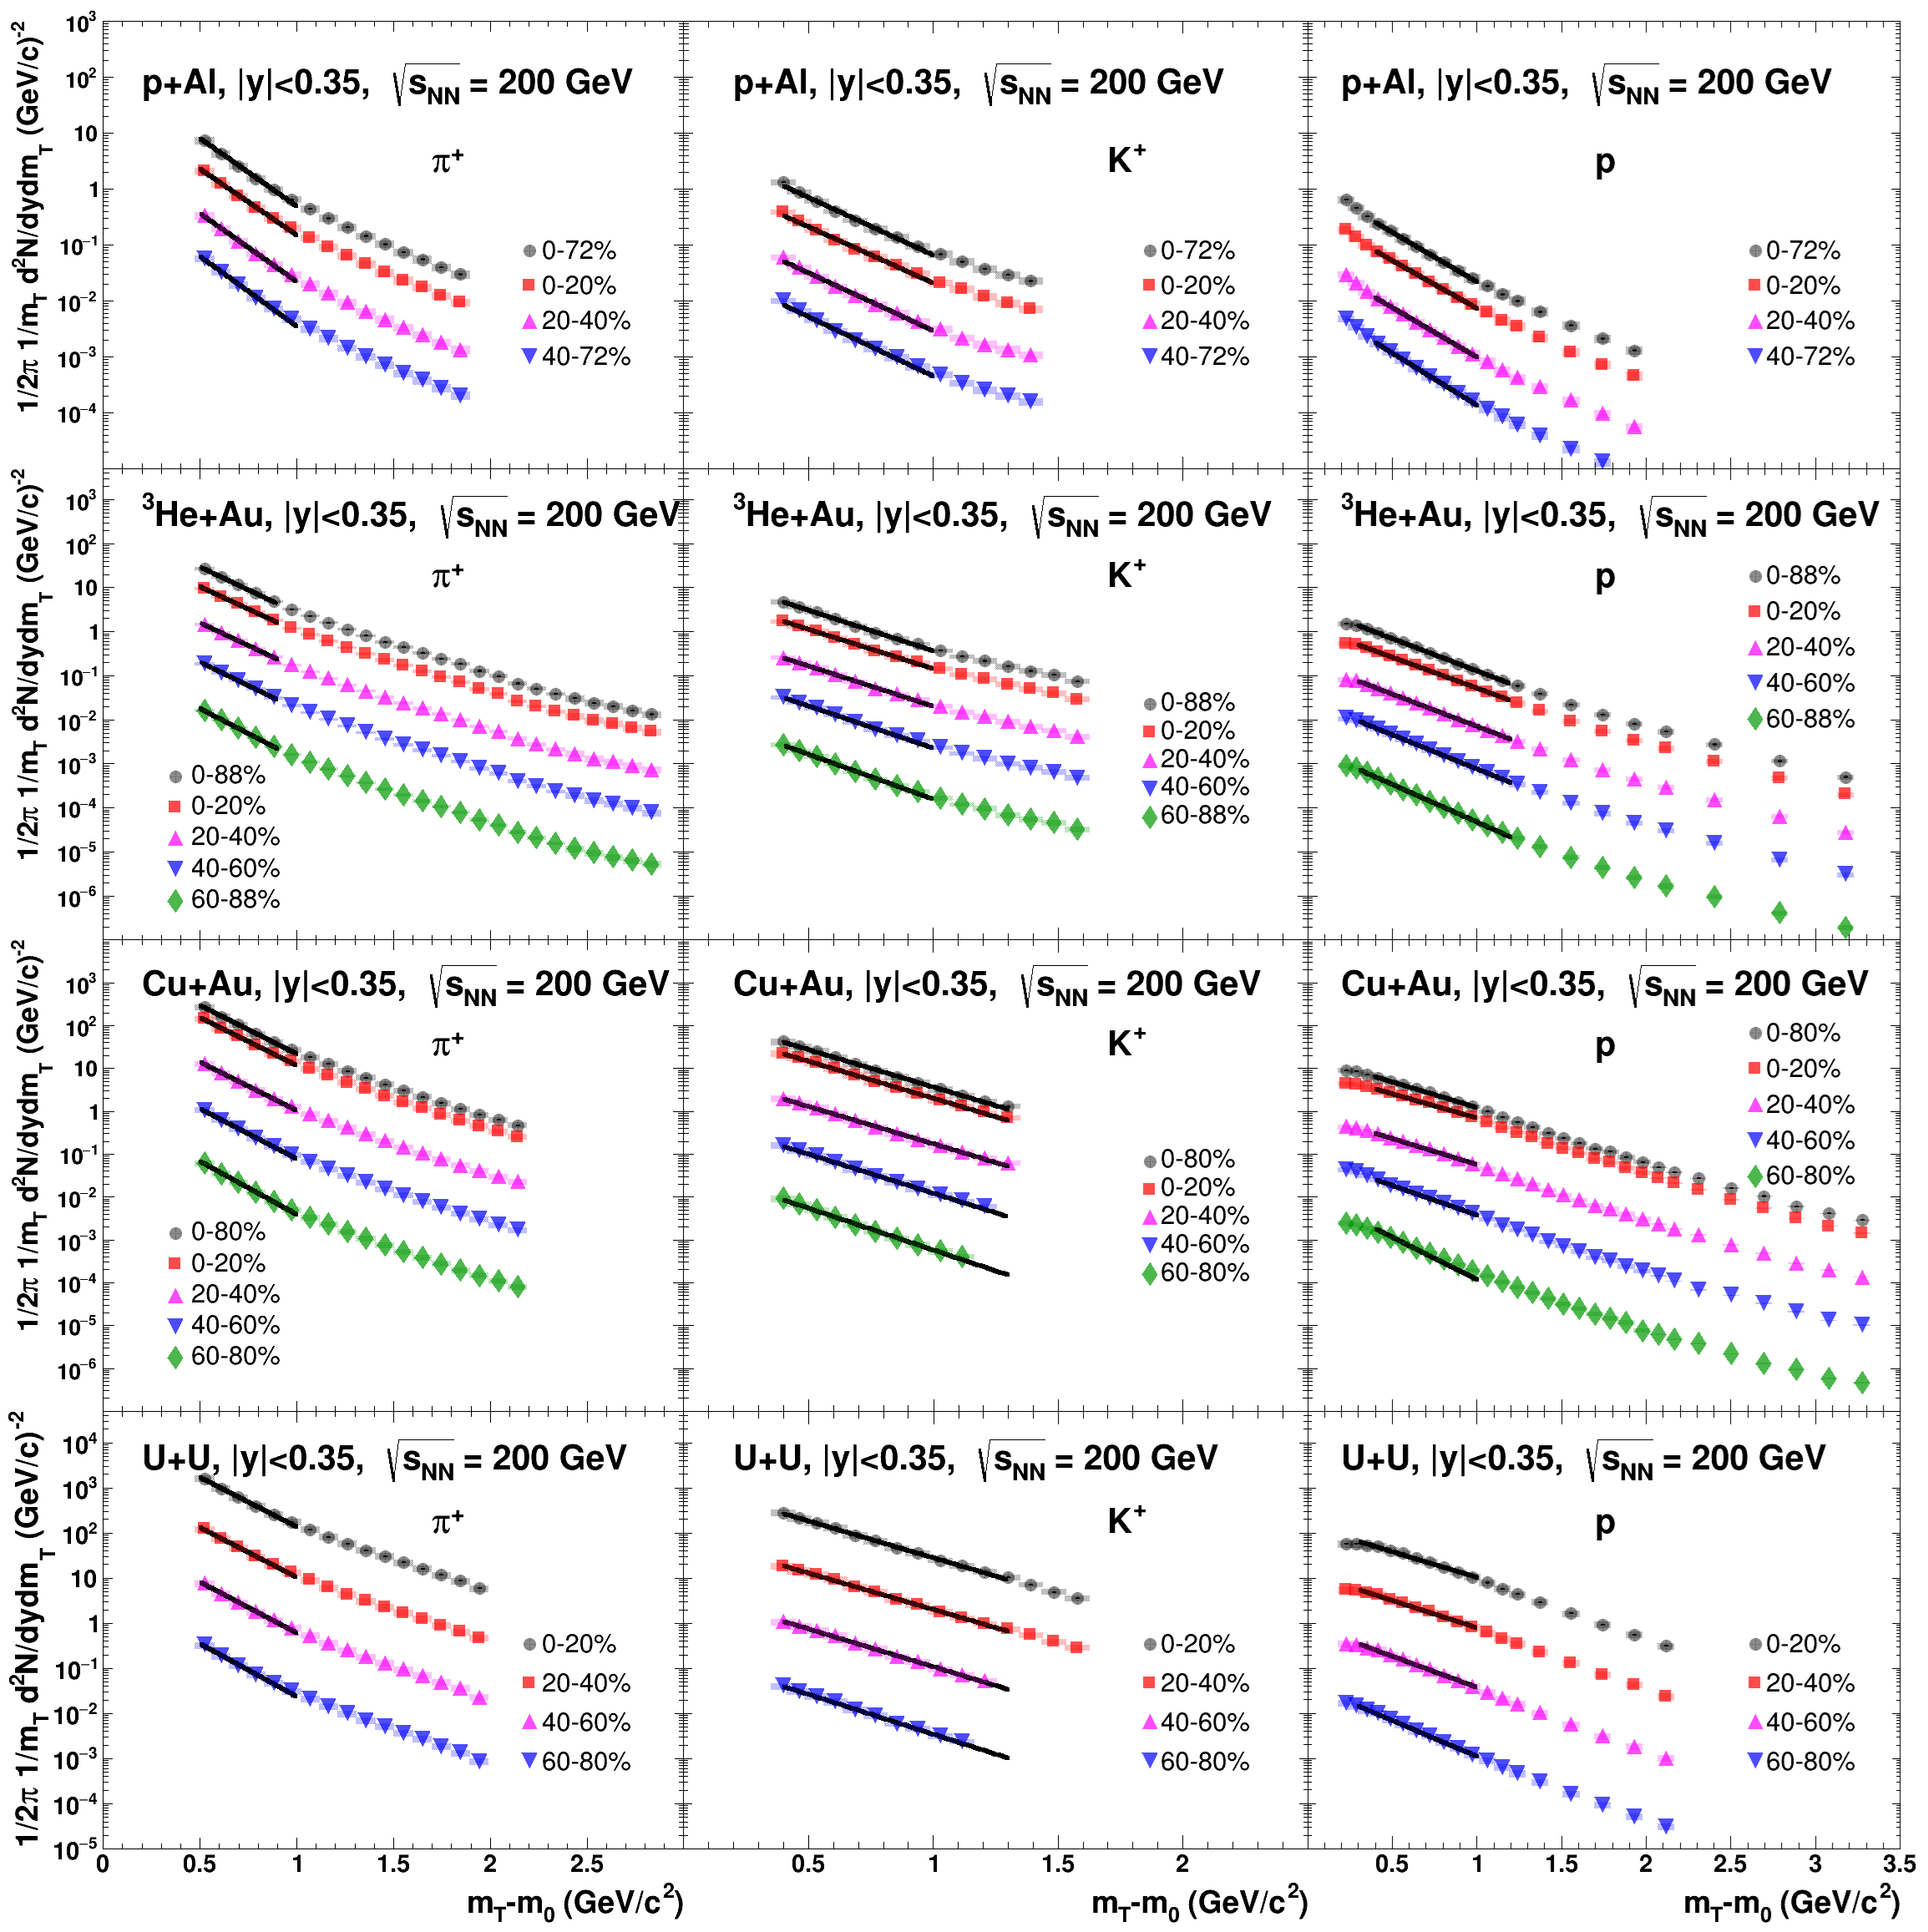
\includegraphics [width=1\linewidth]{Results/spectraDiss_mt_0.png}
	\caption{Инвариантные спектры по поперечному массе, измеренные для положительно заряженных адронов в различных центральностях \pal, \heau, Cu+Au и U+U столкновениях.} 
	\label{img:SpectraMt0}
\end{figure}
\begin{figure}[] 
	\centerfloat
	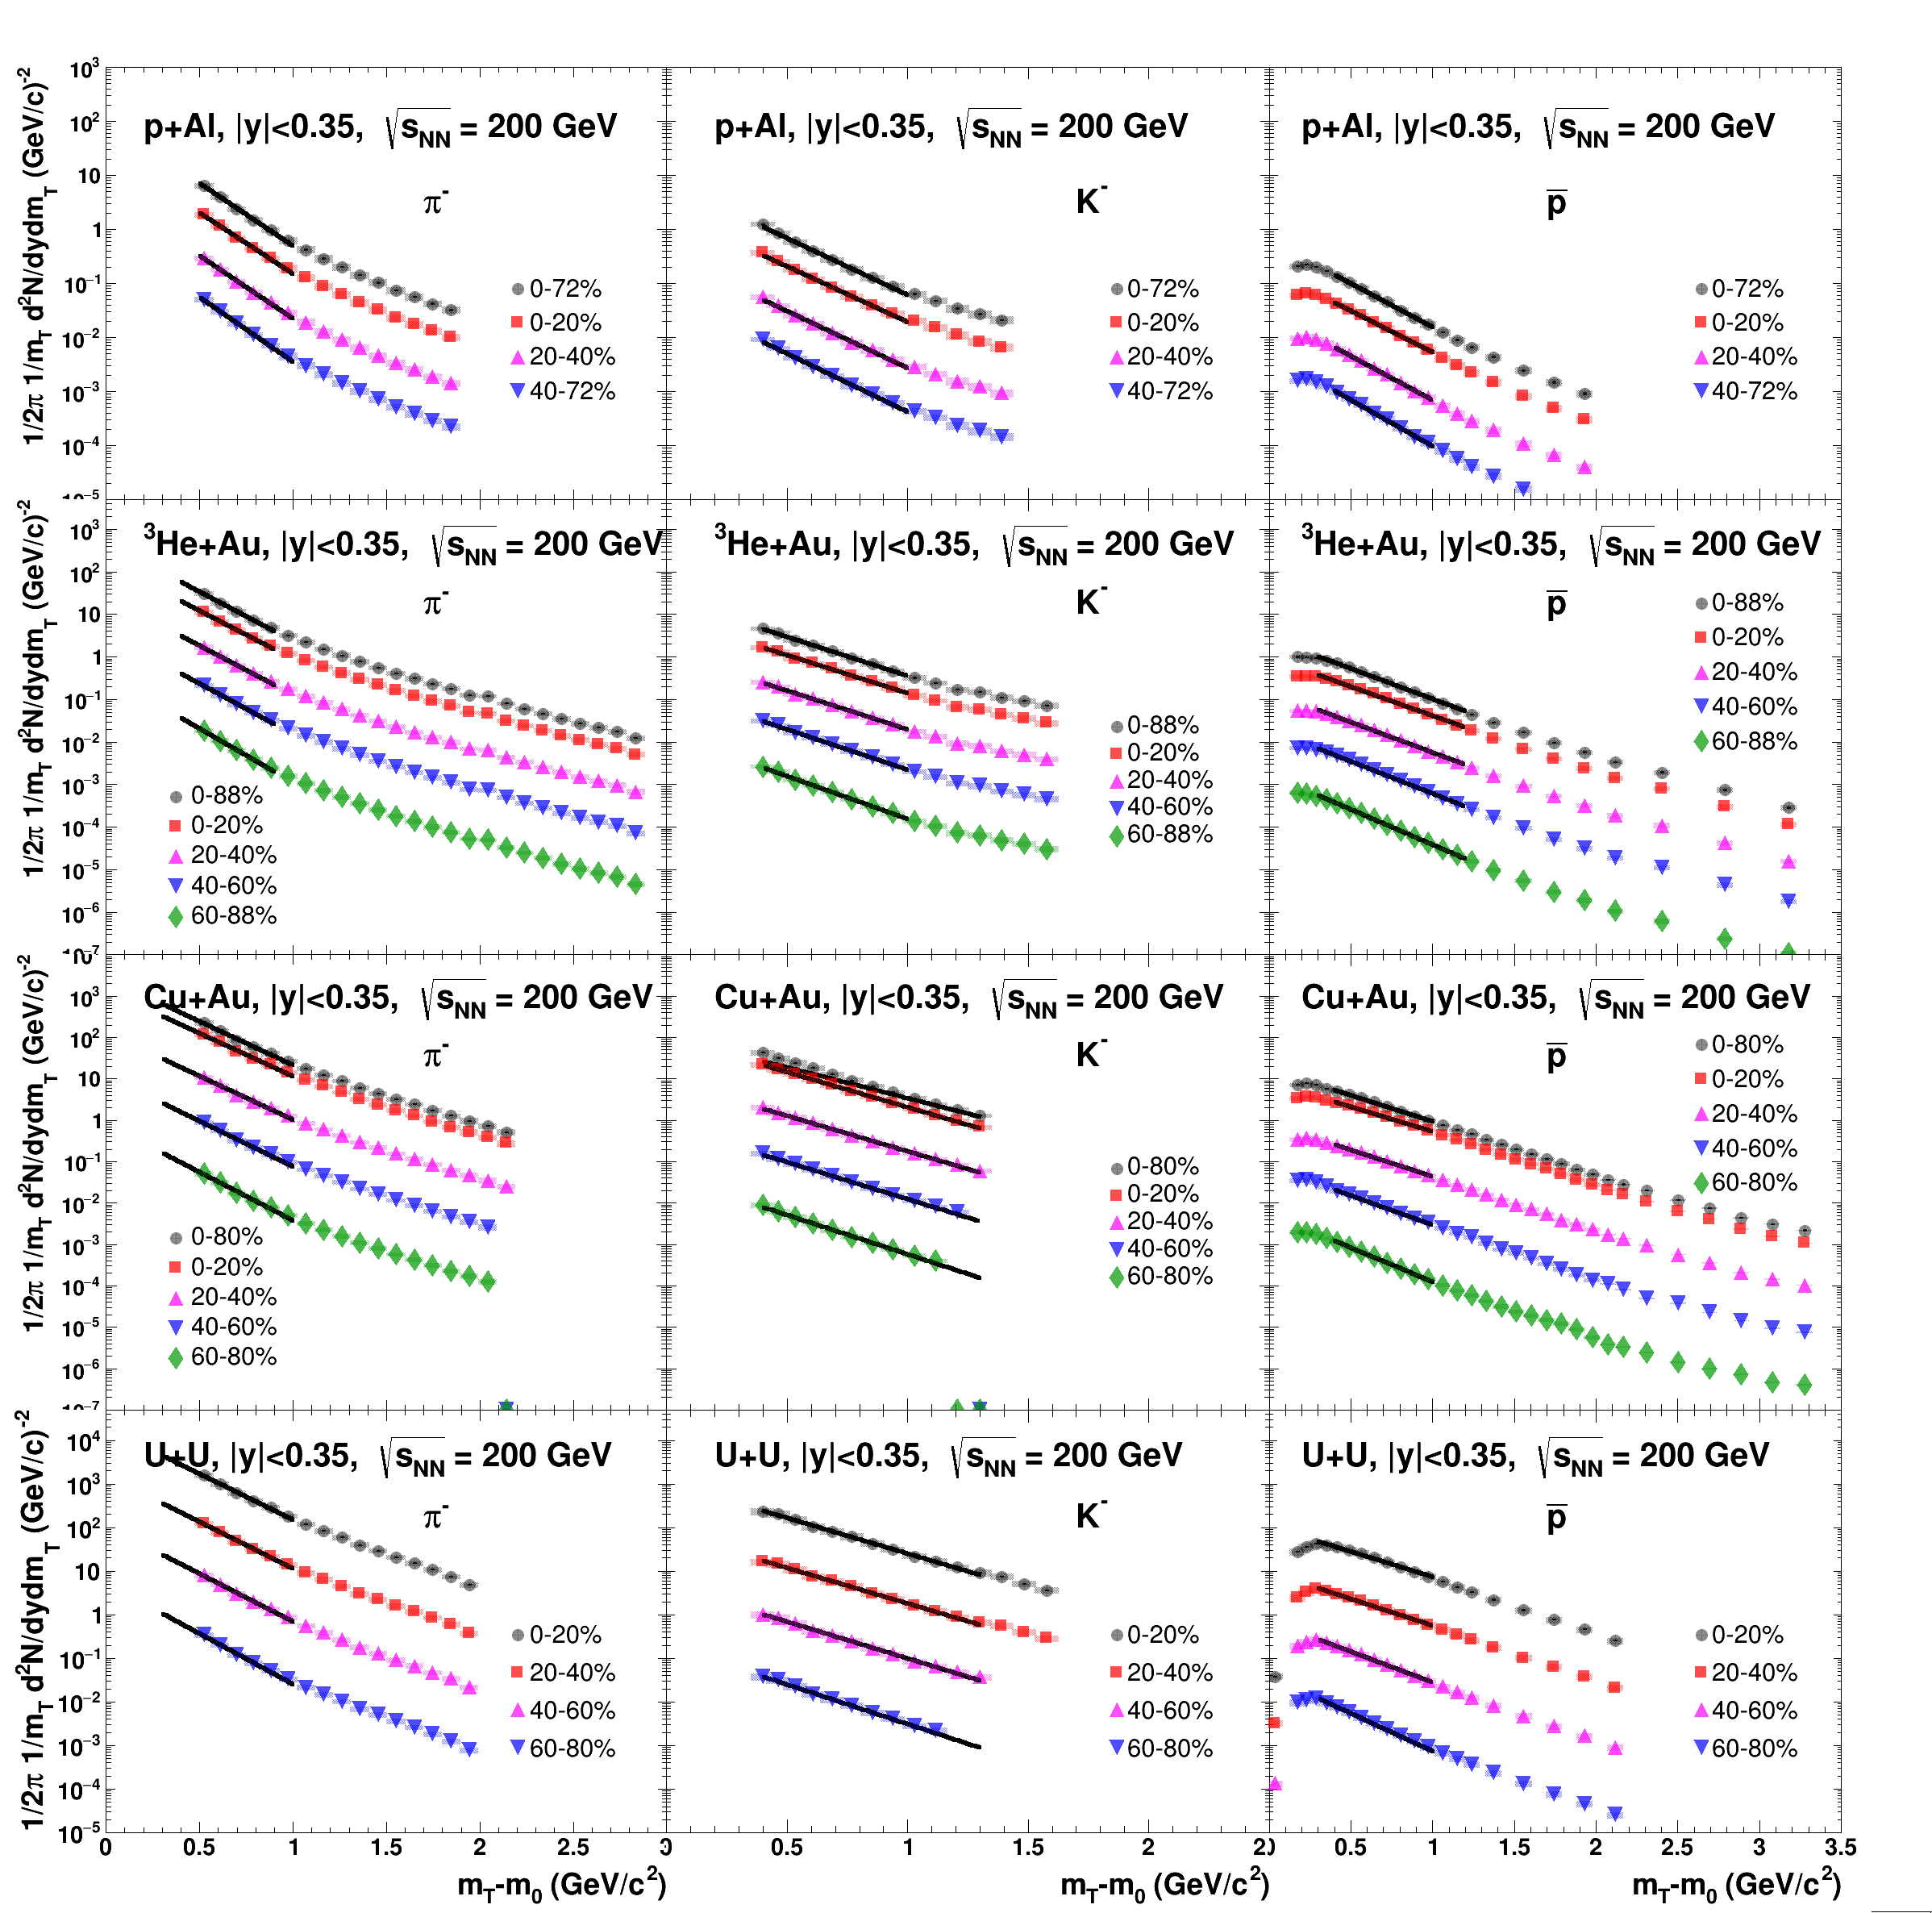
\includegraphics [width=1\linewidth]{Results/spectraDiss_mt_1.png}
	\caption{Инвариантные спектры по поперечному массе, измеренные для отрицательно заряженных адронов в различных центральностях \pal, \heau, Cu+Au и U+U столкновениях.} 
	\label{img:SpectraMt1}
\end{figure}

Полученные параметры обратного наклона аппроксимационных прямых ($T$) приведены в таблицах \ref{table:Tinv_pos}, \ref{table:Tinv_neg} и представлены на рис. \ref{img:Tinv0}, \ref{img:Tinv1} в зависимости от массы ($m_0$) положительно и отрицательно заряженных адронов в различных интервалах центральности столкновений \pal, \heau, Cu+Au, U+U. 
%Значения параметров $T$ увеличиваются с увеличением массы частиц во всех рассматриваемых инервалах центральности всех рассматриваемых систем столкновений.  

\begin{table}[]
	\caption{Значения параметров обратного наклона $T$ (ГэВ/$c^2$), вычисленные для положительно заряженных идентифицируемых адронов (\pip, \Kp, \prot) в столкновениях \pal, \heau, Cu+Au и U+U.}
	\label{table:Tinv_pos}
	
	\begin{tabularx}{\linewidth}
		{
			| >{\centering\arraybackslash}X
			| >{\centering\arraybackslash}X
			| >{\centering\arraybackslash}X
			| >{\centering\arraybackslash}X | }
		\hline
		\Npart     &  \pip & \Kp &\prot   \\ \hline
		\bfseries{\pal}      &     &     &      \\
		3.1 $\pm$ 0.1 &  178.88 $\pm$ 0.35  &  210.69 $\pm$ 0.77   &  --  \\
		4.4 $\pm$ 0.3 &  183.83 $\pm$ 0.28  &  216.10 $\pm$ 1.22   &  -- \\
		3.3 $\pm$ 0.1 &  178.20 $\pm$ 0.32  &  210.05 $\pm$ 1.43   &  --  \\
		1.6 $\pm$ 0.2 &  173.88 $\pm$ 0.46  &  204.74 $\pm$ 1.16   &  --  \\
		\hline
		\bfseries{\heau}       &     &     &      \\
		11.3 $\pm$ 0.5  &  208.70 $\pm$ 0.07  &  235.84 $\pm$ 0.24  & 295.74 $\pm$ 0.20   \\
		21.1 $\pm$ 1.3  &  214.33 $\pm$ 0.11  &  242.57 $\pm$ 0.38  & 309.27 $\pm$ 0.33    \\
		15.4 $\pm$ 0.9  &  209.84 $\pm$ 0.13  &  237.27 $\pm$ 0.44  & 296.44 $\pm$ 0.37  \\
		9.5 $\pm$ 0.6   &  202.71 $\pm$ 0.15  &  227.37 $\pm$ 0.53  & 280.01 $\pm$ 0.44    \\
		4.8 $\pm$ 0.3   &  191.01 $\pm$ 0.18  &  213.44 $\pm$ 0.66  & 254.22 $\pm$ 0.55    \\
		\hline
		\bfseries{Cu+Au}       &     &     &       \\
		70.4 $\pm$ 3.0  &  191.72 $\pm$ 0.01 &  249.33 $\pm$ 0.03 &  363.65 $\pm$ 0.09     \\
		154.8 $\pm$ 4.1 &  194.29 $\pm$ 0.12 &  251.43 $\pm$ 0.04 &  383.85 $\pm$ 0.13     \\
		80.4 $\pm$ 3.3  &  192.07 $\pm$ 0.02 &  249.14 $\pm$ 0.06 &  357.54 $\pm$ 0.16     \\
		34.9 $\pm$ 1.8  &  185.32 $\pm$ 0.03 &  238.05 $\pm$ 0.09 &  313.90 $\pm$ 0.20     \\
		11.5 $\pm$ 1.8  &  175.24 $\pm$ 0.05 &  222.76 $\pm$ 0.18 &  270.86 $\pm$ 0.28     \\
		\hline
		\bfseries{U+U}       &     &     &     \\
		330 $\pm$ 6 &  198.18 $\pm$ 0.02  &  266.49 $\pm$ 0.08  & 382.54 $\pm$ 0.19  \\
		259 $\pm$ 7 &  197.28 $\pm$ 0.04  &  269.42 $\pm$ 0.12  & 358.24 $\pm$ 0.23  \\
		65 $\pm$ 6  &  192.42 $\pm$ 0.06  &  259.69 $\pm$ 0.22  & 314.92 $\pm$ 0.32  \\
		\hline
		
	\end{tabularx}
\end{table}

\begin{table}[]
	\caption{Значения параметров обратного наклона $T$ (ГэВ/$c^2$), вычисленные для отрицательно заряженных идентифицируемых адронов (\pim, \Km, \aprot) в столкновениях \pal, \heau, Cu+Au и U+U.}
	\label{table:Tinv_neg}
	
	\begin{tabularx}{\linewidth}
		{
			| >{\centering\arraybackslash}X
			| >{\centering\arraybackslash}X
			| >{\centering\arraybackslash}X
			| >{\centering\arraybackslash}X | }
		\hline
		
		\Npart     & \pim & \Km & \aprot     \\ \hline
		\bfseries{\pal}      &     &     &     \\
		3.1 $\pm$ 0.1 &  187.36 $\pm$ 0.18  &  206.61 $\pm$ 0.78    &  269.51 $\pm$ 1.25    \\
		4.4 $\pm$ 0.3 &  192.56 $\pm$ 0.29  &  211.25 $\pm$ 1.21 &  275.14 $\pm$ 1.16    \\
		3.3 $\pm$ 0.1 &  186.96 $\pm$ 0.33  &  206.25 $\pm$ 1.46  &  266.62 $\pm$ 2.28    \\
		1.6 $\pm$ 0.2 &  181.99 $\pm$ 0.26  &  201.47 $\pm$ 1.18  &  254.20 $\pm$ 1.82    \\
		\hline
		\bfseries{\heau}       &     &     &      \\
		11.3 $\pm$ 0.5  &  187.25 $\pm$ 0.06  &  236.98 $\pm$ 0.25 &  303.59 $\pm$ 0.24    \\
		21.1 $\pm$ 1.3  &  191.58 $\pm$ 0.09  &  242.91 $\pm$ 0.39  &  317.40 $\pm$ 0.76    \\
		15.4 $\pm$ 0.9  &  188.33 $\pm$ 0.10  &  238.49 $\pm$ 0.46  &295.10 $\pm$ 0.18    \\
		9.5 $\pm$ 0.6   &  182.66 $\pm$ 0.13  &  229.34 $\pm$ 0.55  &  287.12 $\pm$ 0.54    \\
		4.8 $\pm$ 0.3   &  172.40 $\pm$ 0.15  &  215.99 $\pm$ 0.70  &  261.83 $\pm$ 0.66    \\
		\hline
		\bfseries{Cu+Au}       &     &     &         \\
		70.4 $\pm$ 3.0  &  205.41 $\pm$ 0.01  &  253.80 $\pm$ 0.03  & 344.75 $\pm$ 0.08    \\
		154.8 $\pm$ 4.1 &  208.57 $\pm$ 0.01  &  255.85 $\pm$ 0.09  & 365.18 $\pm$ 0.13    \\
		80.4 $\pm$ 3.3  &  205.67 $\pm$ 0.02  &  253.34 $\pm$ 0.05  & 338.92 $\pm$ 0.15    \\
		34.9 $\pm$ 1.8  &  197.72 $\pm$ 0.03  &  243.35 $\pm$ 0.09  & 306.48 $\pm$ 0.20    \\
		11.5 $\pm$ 1.8  &  186.06 $\pm$ 0.05  &  228.90 $\pm$ 0.18  & 263.38 $\pm$ 0.29    \\
		\hline
		\bfseries{U+U}       &     &     &       \\
		330 $\pm$ 6 &  205.84 $\pm$ 0.21  &  265.80 $\pm$ 0.08  &  374.48 $\pm$ 0.21    \\
		259 $\pm$ 7 &  202.39 $\pm$ 0.03  &  266.36 $\pm$ 0.11  &  353.94 $\pm$ 0.26    \\
		65 $\pm$ 6  &  197.74 $\pm$ 0.06  &  257.80 $\pm$ 0.20  &  308.57 $\pm$ 0.35    \\
		\hline
	\end{tabularx}
\end{table}



\begin{table}[]
	\caption{Значения аппроксимационных параметров \To \ и \ut, вычисленные для различных систем столкновений: \pal, \heau, Cu+Au, U+U.}
	\label{table:To_ut}
	
	\begin{tabularx}{\linewidth}
		{
			| >{\centering\arraybackslash}X
			| >{\centering\arraybackslash}X
			| >{\centering\arraybackslash}X
			| >{\centering\arraybackslash}X
			| >{\centering\arraybackslash}X | }
		\hline
		
		\Npart     & $T_{0}^{+}$ & $T_{0}^{-}$  & $\left<u_{t}\right>^{+}$ & $\left<u_{t}\right>^{-}$   \\ \hline
		
		\bfseries{\pal}       &     &     &      &    \\
		3.1$\pm$0.1  &  167.9 $\pm$ 2.1  &  166.4 $\pm$ 15.2  &  0.2 $\pm$ 0.1  &  0.3 $\pm$ 0.1   \\
		4.4$\pm$0.3   &  171 $\pm$ 0.9  &  171.3 $\pm$ 15.9  &  0.2 $\pm$ 0.1  &  0.3 $\pm$ 0.1 \\
		3.3$\pm$0.1  &  167.9 $\pm$ 2.1  &  167.8 $\pm$ 14.3  &  0.2 $\pm$ 0.1  &  0.3 $\pm$ 0.1    \\
		1.6$\pm$0.2  &  164 $\pm$ 4.3  &  163.8 $\pm$ 11.2  &  0.2 $\pm$ 0.1  &  0.3 $\pm$ 0.1    \\
		\hline
		\bfseries{\heau}       &     &     &      &    \\
		11.3$\pm$0.5  &  188.9 $\pm$ 10.2  &  166.2 $\pm$ 1.7  &  0.3 $\pm$ 0.1  &  0.3 $\pm$ 0.1    \\
		21.1$\pm$1.3  &  193 $\pm$ 12.4  &  166.4 $\pm$ 3.2  &  0.3 $\pm$ 0.1  &  0.3 $\pm$ 0.1    \\
		15.4$\pm$0.9  &  188.9 $\pm$ 9.8  &  167.5 $\pm$ 1.2  &  0.3 $\pm$ 0.1  &  0.3 $\pm$ 0.1    \\
		9.5$\pm$0.6  &  185 $\pm$ 8.5  &  164.6 $\pm$ 0.2  &  0.3 $\pm$ 0.1  &  0.3 $\pm$ 0.1    \\
		4.8$\pm$0.3  &  177 $\pm$ 4.9  &  158.3 $\pm$ 3.4  &  0.2 $\pm$ 0.1  &  0.3 $\pm$ 0.1    \\
		\hline
		\bfseries{Cu+Au}       &     &     &      &    \\
		70.4$\pm$3.0 &  153.9 $\pm$ 16.6  &  176 $\pm$ 11.9  &  0.4 $\pm$ 0.1  &  0.4 $\pm$ 0.1 \\
		154.8$\pm$4.1  &  150 $\pm$ 23.9  &  172.8 $\pm$ 19.7  &  0.4 $\pm$ 0.1  &  0.4 $\pm$ 0.1    \\
		80.4$\pm$3.3  &  157 $\pm$ 14.5  &  178.1 $\pm$ 10.2  &  0.4 $\pm$ 0.1  &  0.4 $\pm$ 0.1    \\
		34.9$\pm$2.9  &  160.9 $\pm$ 3.8  &  177.7 $\pm$ 2.3  &  0.4 $\pm$ 0.1  &  0.3 $\pm$ 0.1    \\
		11.5$\pm$1.8 &  159.9 $\pm$ 4.5  &  175.8 $\pm$ 7.5  &  0.3 $\pm$ 0.1  &  0.3 $\pm$ 0.1    \\
		\hline
		\bfseries{U+U}       &     &     &      &    \\
		330$\pm$6 &  159.9 $\pm$ 12  &  170.8 $\pm$ 13.2  &  0.4 $\pm$ 0.1  &  0.4 $\pm$ 0.1  \\
		259$\pm$7 &  168.9 $\pm$ 0.6  &  174.7 $\pm$ 2.9  &  0.4 $\pm$ 0.1  &  0.4 $\pm$ 0.1    \\
		65$\pm$6   &  175.9 $\pm$ 11.4  &  182.6 $\pm$ 9.6  &  0.3 $\pm$ 0.1  &  0.3 $\pm$ 0.1 \\
		\hline
	\end{tabularx}
\end{table}

В рамках модели термодинамического расширения зависимости \cite{Thermal1, Coalescence_models, ToutModels} $T$($m_0$) в свою очередь могут быть аппроксимированы (см. раздел \ref{sectRes_spectra}) линейной функцией с параметрами \To \ и \ut \cite{PPG026}:
\begin{equation}
	\label{eq:InvSlope}
	T = T_0 +m_0 \left< u_t\right>^2
\end{equation}
где параметр $T_0$ интерпретируется как температура при которой достигается химическое равновенисие КГП, а \ut \ -- как поперечная скорость коллективного движения партонов. 
%Также параметр $T_0$ можно интерпретировать как линейную экстраполяцию параметра обратного наклона $T$ к нулевой массе $m=0$.
Линейная аппроксимация зависимости $T(m_0)$ с использованием уравнения. \ref{eq:InvSlope} изображена на рисунках \ref{img:Tinv0}, \ref{img:Tinv1} пунктирными линиями.

\begin{figure}[] 
	\centerfloat
	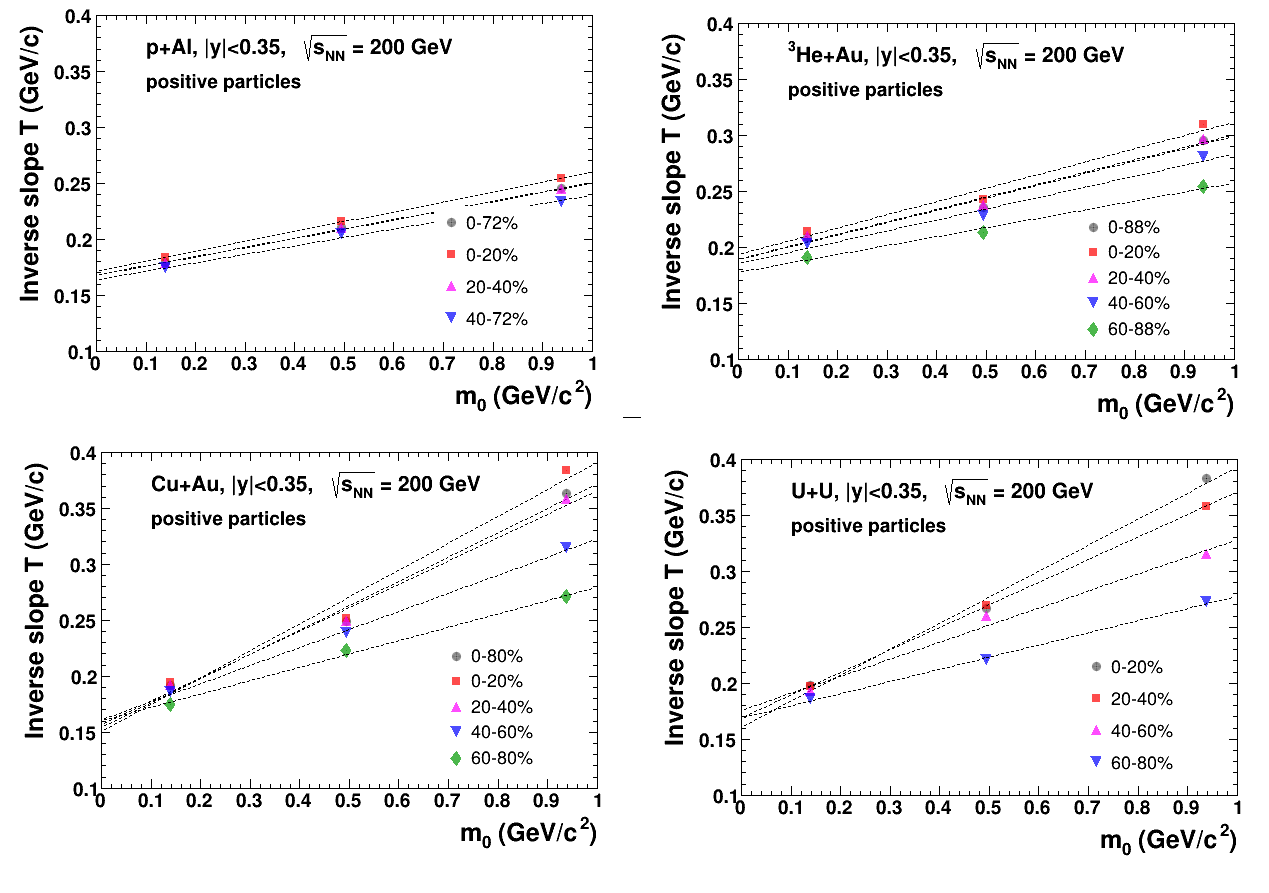
\includegraphics [width=0.85\linewidth]{Results/Tgr0.png}
	\caption{Зависимость величины параметра обратного наклона $T$ от массы \pip, \Kp, \prot \ в различных центральностях \pal, \heau, Cu+Au и U+U столкновениях.} 
	\label{img:Tinv0}
\end{figure}
\begin{figure}[] 
	\centerfloat
	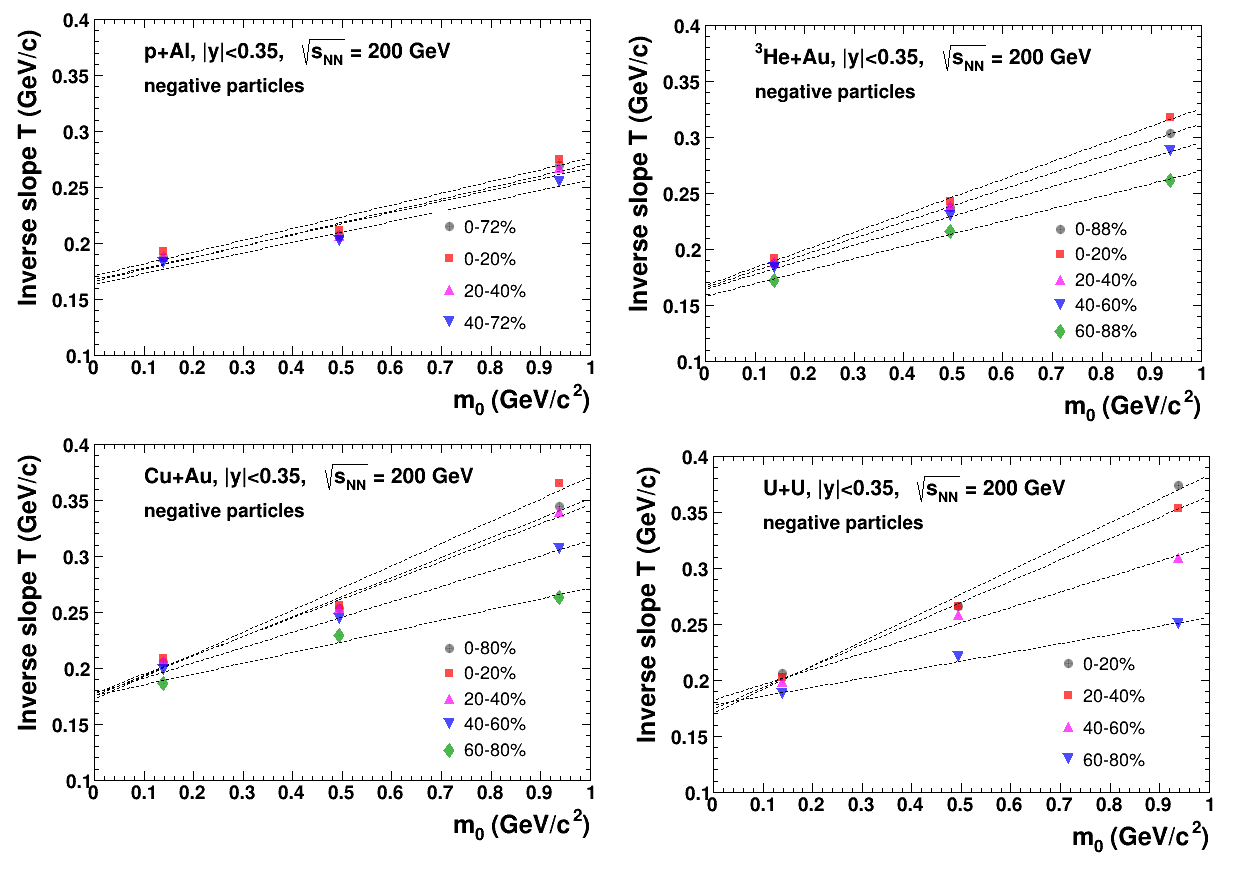
\includegraphics [width=0.85\linewidth]{Results/Tgr1.png}
	\caption{Зависимость величины параметра обратного наклона $T$ от массы \pim, \Km, \aprot \ в различных центральностях \pal, \heau, Cu+Au и U+U столкновениях.} 
	\label{img:Tinv1}
\end{figure}


\begin{figure}[ht]
	\centerfloat{
		\hfill
		\subcaptionbox{ }{
			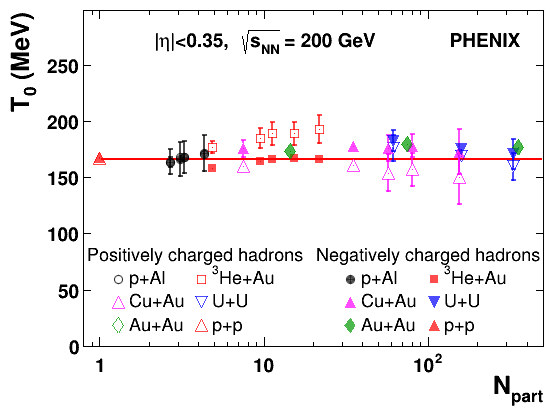
\includegraphics[width=0.45\linewidth]{Results/T0_Npart.png}
		}
		\hfill
		\subcaptionbox{ }{
			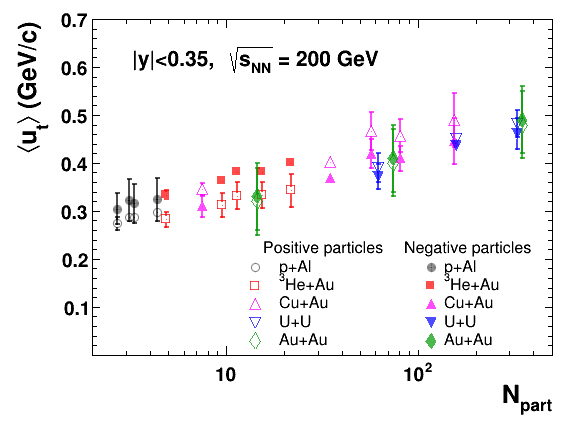
\includegraphics[width=0.45\linewidth]{Results/ut_Npart.png}}
		\hfill
	}
	\caption{Зависимость а) температуры вымораживания $T_0$ и  б) скорости поперечного потока $u_T$ от количество нуклонов участников \Npart.}
	\label{fig:TuNpart}
\end{figure}

Полученные значения $T_0$ и $\left< u_t \right>$ приведены в таблице \ref{table:To_ut}, а также представлены на рис.\ref{fig:TuNpart} в зависимости от значений \Npart. Из приведенных таблиц \ref{table:To_ut} и рис.\ref{fig:TuNpart} видно, что величины параметра $T_0$ не зависят от значений \Npart, в то время как величины $\left< u_t \right>$ увеличиваются с ростом \Npart. Данный результат находится в соответствии с гидродинамической картиной столкновения и моделью термодинамического расширения \cite{HydroPartonicCascade}.

\section{Сравнение с результатами моделирования} \label{sect5_spectra}

Для более глубокого анализа полученных экспериментальных данных, было осуществлено моделирование \pal, \heau, Cu+Au столкновений при $\sqrt{s_{NN}}$ = 200 ГэВ и U+U столкновений при $\sqrt{s_{NN}}$ = 193 ГэВ с помощью программных пакетов PYTHIA/ANGANTYR 8.3 \cite{pythia} и AMPT \cite{AMPT}.
Принципиальное различие данных программных пакетов состоит в различных моделях адронизации партонов: пакет PYTHIA/ANGANTYR 8.3 \cite{pythia} реализует модель адронизации Лунда \cite{FragmentationLund}, в то время как AMPT \cite{AMPT} в версии с плалением струн реализует рекомбинационную модель адронизации \cite{Recombination1, Recombination2}.

\begin{comment}
	\subsection{PYTHIA8}
	\label{subsect5_pythia}
	PYTHIA 8.3 - программный пакет, основанный на методе Монте-Карло, предназначенный для моделирования ультрорелятивистских столкновений, основанный на теоретических расчетах КХД, а также модели фрагментации Лунда.
	
	Процесс моделирования столкновения в PYTHIA 8.3 состоит из трех основных этапов: первый этап - моделирование жестких процессов, второй этап - моделирование партонных взаимодействий и третий этап - моделирование адронных взаимодействий.
	
	На первом этапе происходит моделирование процесса жесткого рассеяния и рождения короткоживущих резонансов. Жесткие рассеяния частиц моделируются согнласно расчетам  пертурбативной КХД.
	
	На этапе партонных взаимодействий происходит моделирование излучения в начальном и конечном состоянии. Также на данном уровне реализованы многопартонные взаимодействия и происходит обработка нуклонов-спектаторов. На завершающей стадии партонного уровня событие представляет собой реалистичную партонную структуру, включающую струи и  основноое жесткое взаимодействие. 
	
	На завершающем адронном этапе осуществляется объединение партонов в синглетные по цвету состояния. В PYTHIA 8.3 процесс адронизации описывается с помощью КХД струн, фрагментирующимися в адроны. Также на адронном уровне реализуется распад нестабильных адронов и адронное рассеяние. Физические модели адронизации обычно являются непертурбативными, и поэтому требуют моделирования и настройки параметров. Выход на адронном уровне является реалистичным событием. поскольку его можно наблюдать в детекторе.
	
	Модель Лунда фрагментации струн широко используется для описания
	процесса адронизации $p+p$ -столкновений и для выполнения расчетов КХД. В 1997 году на основе этой модели был создан программный пакет PYTHIA, целью которого является моделирование процесса взаимодействия протонов при высокой энергии.
	/* Может начать с модели лунда? */
	
	Таким образом, программный пакет PYTHIA не учитывает возможности образования КГП.
	
	%Программный пакет PYTHIA 8.3 \cite{pythia} широко используется для генерации событий в высокоэнергетических столкновениях частиц, где эффекты сильной ядерной силы, управляемые квантовой хромодинамикой (КХД), имеют большое значение. PYTHIA включает в себя полный набор подробных физических моделей для эволюции от процесса жесткого рассеяния нескольких тел до сложного многочастичного конечного состояния. Часть физики была строго выведена из теории, в то время как другие части основаны на феноменологических моделях, с параметрами определенными согласно критерию соответствия экспериментальным данным. Основные задачи, выполняемые программой, включают исследования экспериментальных последствий теоретических гипотез, интерпретацию экспериментальных данных - включая оценку систематических неопределенностей и разворачивания - разработка стратегий поиска, а также исследования конструкции и характеристик детекторов. Он также играет важную роль в качестве универсального сосуда для изучения новых теоретических идей и новых алгоритмических подходов, начиная от незначительных пользовательских модификаций и заканчивая полноценной разработкой новых физических моделей.
	
	\subsection{AMPT}
	\label{subsect5_AMPT}
	Одна из основных задач экспериментов по столкновению тяжелых ионов состоит в изучении кварк-глюонной структуры ядерной материи и возможности перехода от адронной материи к КГП.  
	Адронная струя образуется несколькими элементарными частицами, летящими в одном направлении в узком конусе. Физическая причина образования струи — адронизация кварка или глюона с большой энергией (намного большей, чем масса пиона).
	Концепция струй свзяана с жесткими партонными рассеяниями и играет важную роль в столкновениях релятивистских ионов. Эксперименально струи измеряются как адронные кластеры, чья поперечная энергия может быть измерена с помощью калориметров. 
	Однако, когда поперечная энергия струи становится меньше $E_{T}<5$ ГэВ, ее экспериментальное выделение от фоновых событий становится крайне трудной задачей. Не смотря на это, при $E_{T}<5$ ГэВ согласно КХД  жесткие рассеяния продолжают играть существенную роль и могут быть вычеслены в рамках пертурбативной КХД.  Согласно теоретическим оценкам, в столкновении тяжелых ионов министруи несут 50\%-80\% всех поперечной энергии столкновения. 
	Генератор HIJING разработан для моделирования столкновений релятивистских ионов и теоретической оценки влияния министруй на измеряемые эффекты, в том числе на эффекты, связанные с образованием КГП.
	
	\begin{figure}[] 
		\centerfloat
		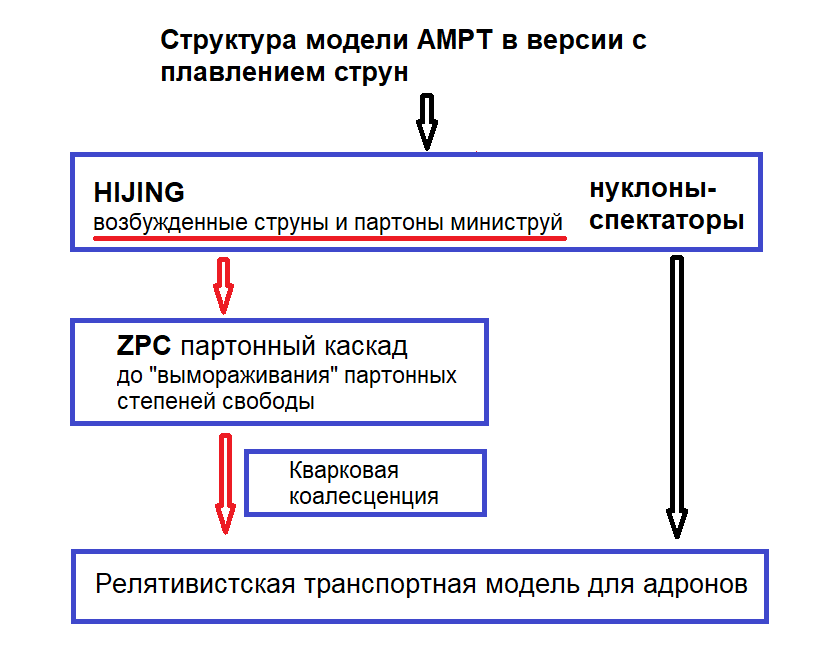
\includegraphics [width=0.5\linewidth]{Simulation/AMPT_SM.png}
		\caption{Иллюстрация структуры программного пакета AMPT в версии с плавлением струн} 
		\label{img:AMPT_sm}
	\end{figure}
	
	К моменту начала фазы адронизации, в столкновении присутствуют струны,  и партоны министруй.  
	Партоны министруй, образованных в жестких процессах, перед фрагментацией в адроны могут рассеиваться. Поскольку количество жестких столкновений в столкновении A+A примерно равно $A^{4/3}$ и растет с увеличением энергии столкновения, в то время как количество струн примерно равно A, влияние министруй увеличивается с ростом энергий. Однако для центральных столкновений Au+Au даже при 200 A ГэВ партоны министруй несут лишь около 1/3 суммарного поперечной энергии, поэтому влияние партонного рассеяния на конечную множественность частиц и спектры довольно мало 
	Приведенная выше картина сосуществования партонов и струн на начальной стадии столкновений тяжелых ионов высоких энергий вызывает сомнения, когда плотность энергии намного выше критической плотности для фазового перехода КХД. В этом случае ожидается, что струны расплавятся в партонные степени свободы. 
	И транспортная модель, и подход КХД высокой плотности предсказывают, что начальная плотность энергии образовавшегося вещества в центральных столкновениях Au+Au на RHIC более чем на порядок превышает критическую плотность энергии ($\sim$1 ГэВ/фм$^{3}$). Таким образом, сохранение струн в области высокой плотности энергии приводит к недооценке партонных эффектов в этих столкновениях. 
	Чтобы смоделировать плавление струны в областях с высокой плотностью энергии до партонов, модель AMPT модифицируется следующим образом. После моделирования начальных условий с помощью пакета HIJING (с выключенным эффектом гашения струй), происходит фрагментация струй в адроны с помощью пакета PYTHIA8, используещего модель Лунда, а затем образовавшиеся адроны конвертируются в партоны в соответствии с их ароматом и спином.
	Релятивиствские эффекты добавлены в модель путем введения времени формирования партонов, образующих министруи, которое зависит от их четырехимульса. 
	
	После того, как партоны перестают взамодействовать, начинается процесс их адрониации путем коалесценции. Модель коалесценции подразумевает, что два партона, находящихся рядом в фазовом пространстве формируют мезон, в то время как 3 кварка, находящихся рядом в фазовом просторанстве формируют барион. Поскольку инвариантная масса объединенных партонов формирует непрерывный 
	\subsection{Результаты}
	
\end{comment}
На рис. \ref{img:Ratio_same_sym} представлено сравнение значений $\pi^{-}/\pi^{+}$, $K^{-}/K^{+}$, $\bar{p}/p$, измеренных в $p$+Al, \heau, Cu+Au столкновениях при энергии 200 ГэВ и U+U столкновениях при энергии 192 ГэВ с предсказанями моделей PYTHIA/ANGANTYR и AMPT. Величины отношений $\pi^{-}/\pi^{+}$, $K^{-}/K^{+}$, $\bar{p}/p$, полученные как с помощью программного пакета AMPT в версии с плавлением струн, так и с помощью программного пакета PYTHIA/ANGANTYR не проявляют значимую зависимость от поперечного импульса и центральности. Полученные результаты моделирования совпадают как с экспериментальными данными, так и с предсказаниями термодинамической модели \cite{PPG026, ThermalisationRHIC}.

На рис. \ref{img:Ratio_LargeP2PI_sym}-\ref{img:Ratio_SmallK2PI_sym} представлены зависимости отношений $K^{+}/\pi^{+}$, $K^{-}/\pi^{-}$, $p/\pi^{+}$, $\bar{p}/\pi^{-}$ от поперечного импульса, измеренные в \pal, \heau, Cu+Au и U+U столкновениях, а также аналогичные зависимости, полученные с помощью программного пакета АMPT и  программного пакета PYTHIA/ANGANTYR.
Величины отношений выходов $K^{+}/\pi^{+}$, $K^{-}/\pi^{-}$ проявляют слабую зависимость от центральности и совпадают с экспериментальными данными в пределах погрешностей. 

На основе результатов, представленных на рис.\ref{img:Ratio_LargeP2PI_sym} и рис.\ref{img:Ratio_SmallP2PI_sym} было установлено, что:

\begin{enumerate}
\item Предсказания значений $p/\pi^{+}$ и $\bar{p}/\pi^{-}$ моделью PYTHIA/ANGANTYR во всех системах столкновений (\pal, \heau, Cu+Au, U+U) оказываются близки к результатам, полученным в \pp столкновениях. 
\item Модель AMPT позволяет качественно (но не количественно) описать рост значений $p/\pi^{+}$ и $\bar{p}/\pi^{-}$, наблюдаемый в эксперименте в столкновениях, характеризующихся значениями $N_{part} \gtrsim 10$, а также зависимость этих значений от центральности. К столкновениям с $N_{part} \gtrsim 10$ относятся столкновения центральные \heau, Cu+Au и U+U столкновения.
\item Величины $p/\pi^{+}$ и $\bar{p}/\pi^{-}$, полученные с помощью модели AMPT, численно не совпадают с экспериментально измеренными.
\item В системах столкновений, характеризующихся малыми значениями \Npart \ ($N_{part} \lesssim 10$) значения $p/\pi^{+}$ и $\bar{p}/\pi^{-}$, полученные с помощью рекомбинационной модели, совпадают с предсказаниями модели фрагментации в пределах погрешностей. К столкновениям с \Npart $\lesssim 10$ относятся столкновения \pal, а также периферические столкновения \heau, Cu+Au и U+U.
\end{enumerate}

Количество барионов и мезонов, пропорционально поперечному размеру КГП на стадии адронизации \cite{Thermal2}. Таким образом, можно сделать вывод, что объем образующейся в столкновении КГП, увеличивается с ростом центральнсти столкновения и, соответственно, с ростом \Npart. Совпадение предсказаний рекомбинационной модели и модели фрагментации  в столкновениях с $N_{part} \lesssim 10$ может свидетельствовать о недостаточности объема образующейся КГП для наблюдаемого увеличения выхода барионов. 
На основании вышеизложенного сделан вывод о том, что в стокновениях, характеризующихся значениями $N_{part} \lesssim 10$ преобладает механизм фрагментации. При этом вклад рекомбинационного механизма усиливается с ростом \Npart, вызывая наблюдаемое увеличение выхода барионов. Тем не менее, модель рекомбинации, реализованная в пакете AMPT, не позволяет численно описать увеличение выходов протонов.

\begin{figure}[] 
	\centerfloat
	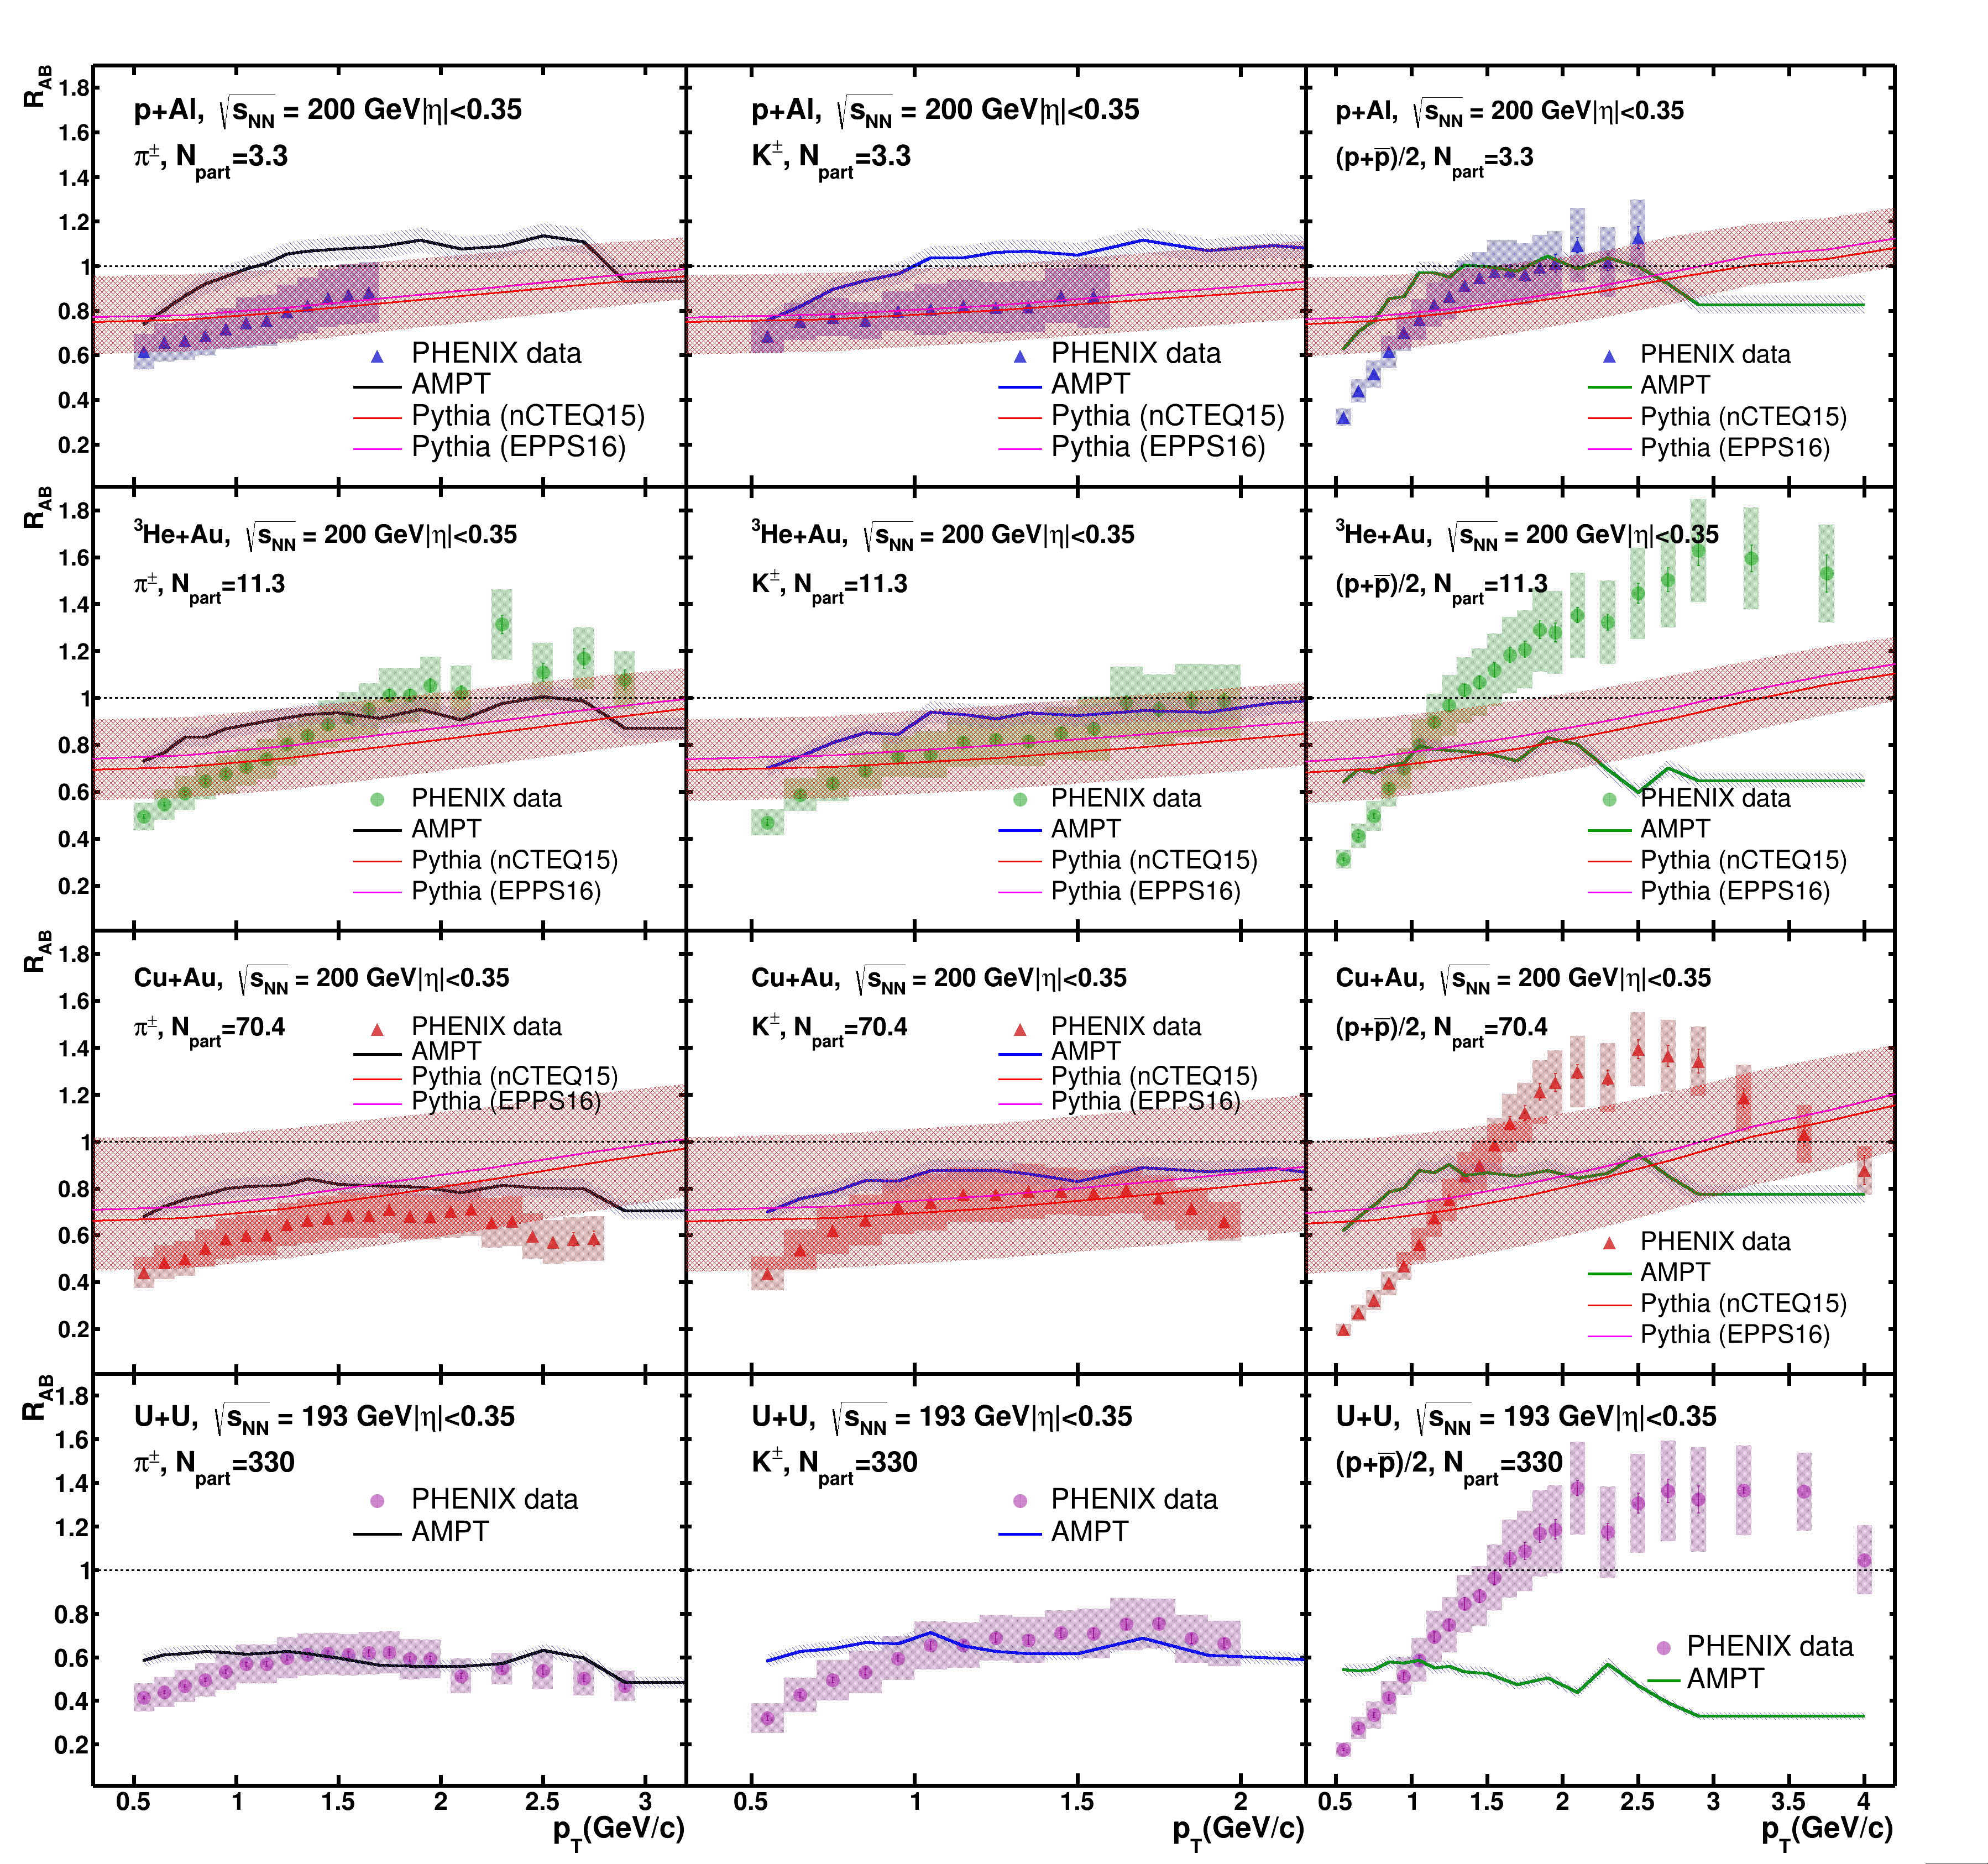
\includegraphics [width=1\linewidth]{Simulation/RAA_AMPT_Pythia.png}
	\caption{Сравнение факторов ядерной модификации (\rab), полученных для \pipm, \Kpm, \prot \ b \aprot \ в рамках фрагментационной (Pythia8) и рекомбинационной (AMPT) моделей, с экспериментальными результатами в различных центральностях \pal, \heau, Cu+Au и U+U столкновений. } 
	\label{img:RAA_sym}
\end{figure}

\begin{figure}[] 
	\centerfloat
	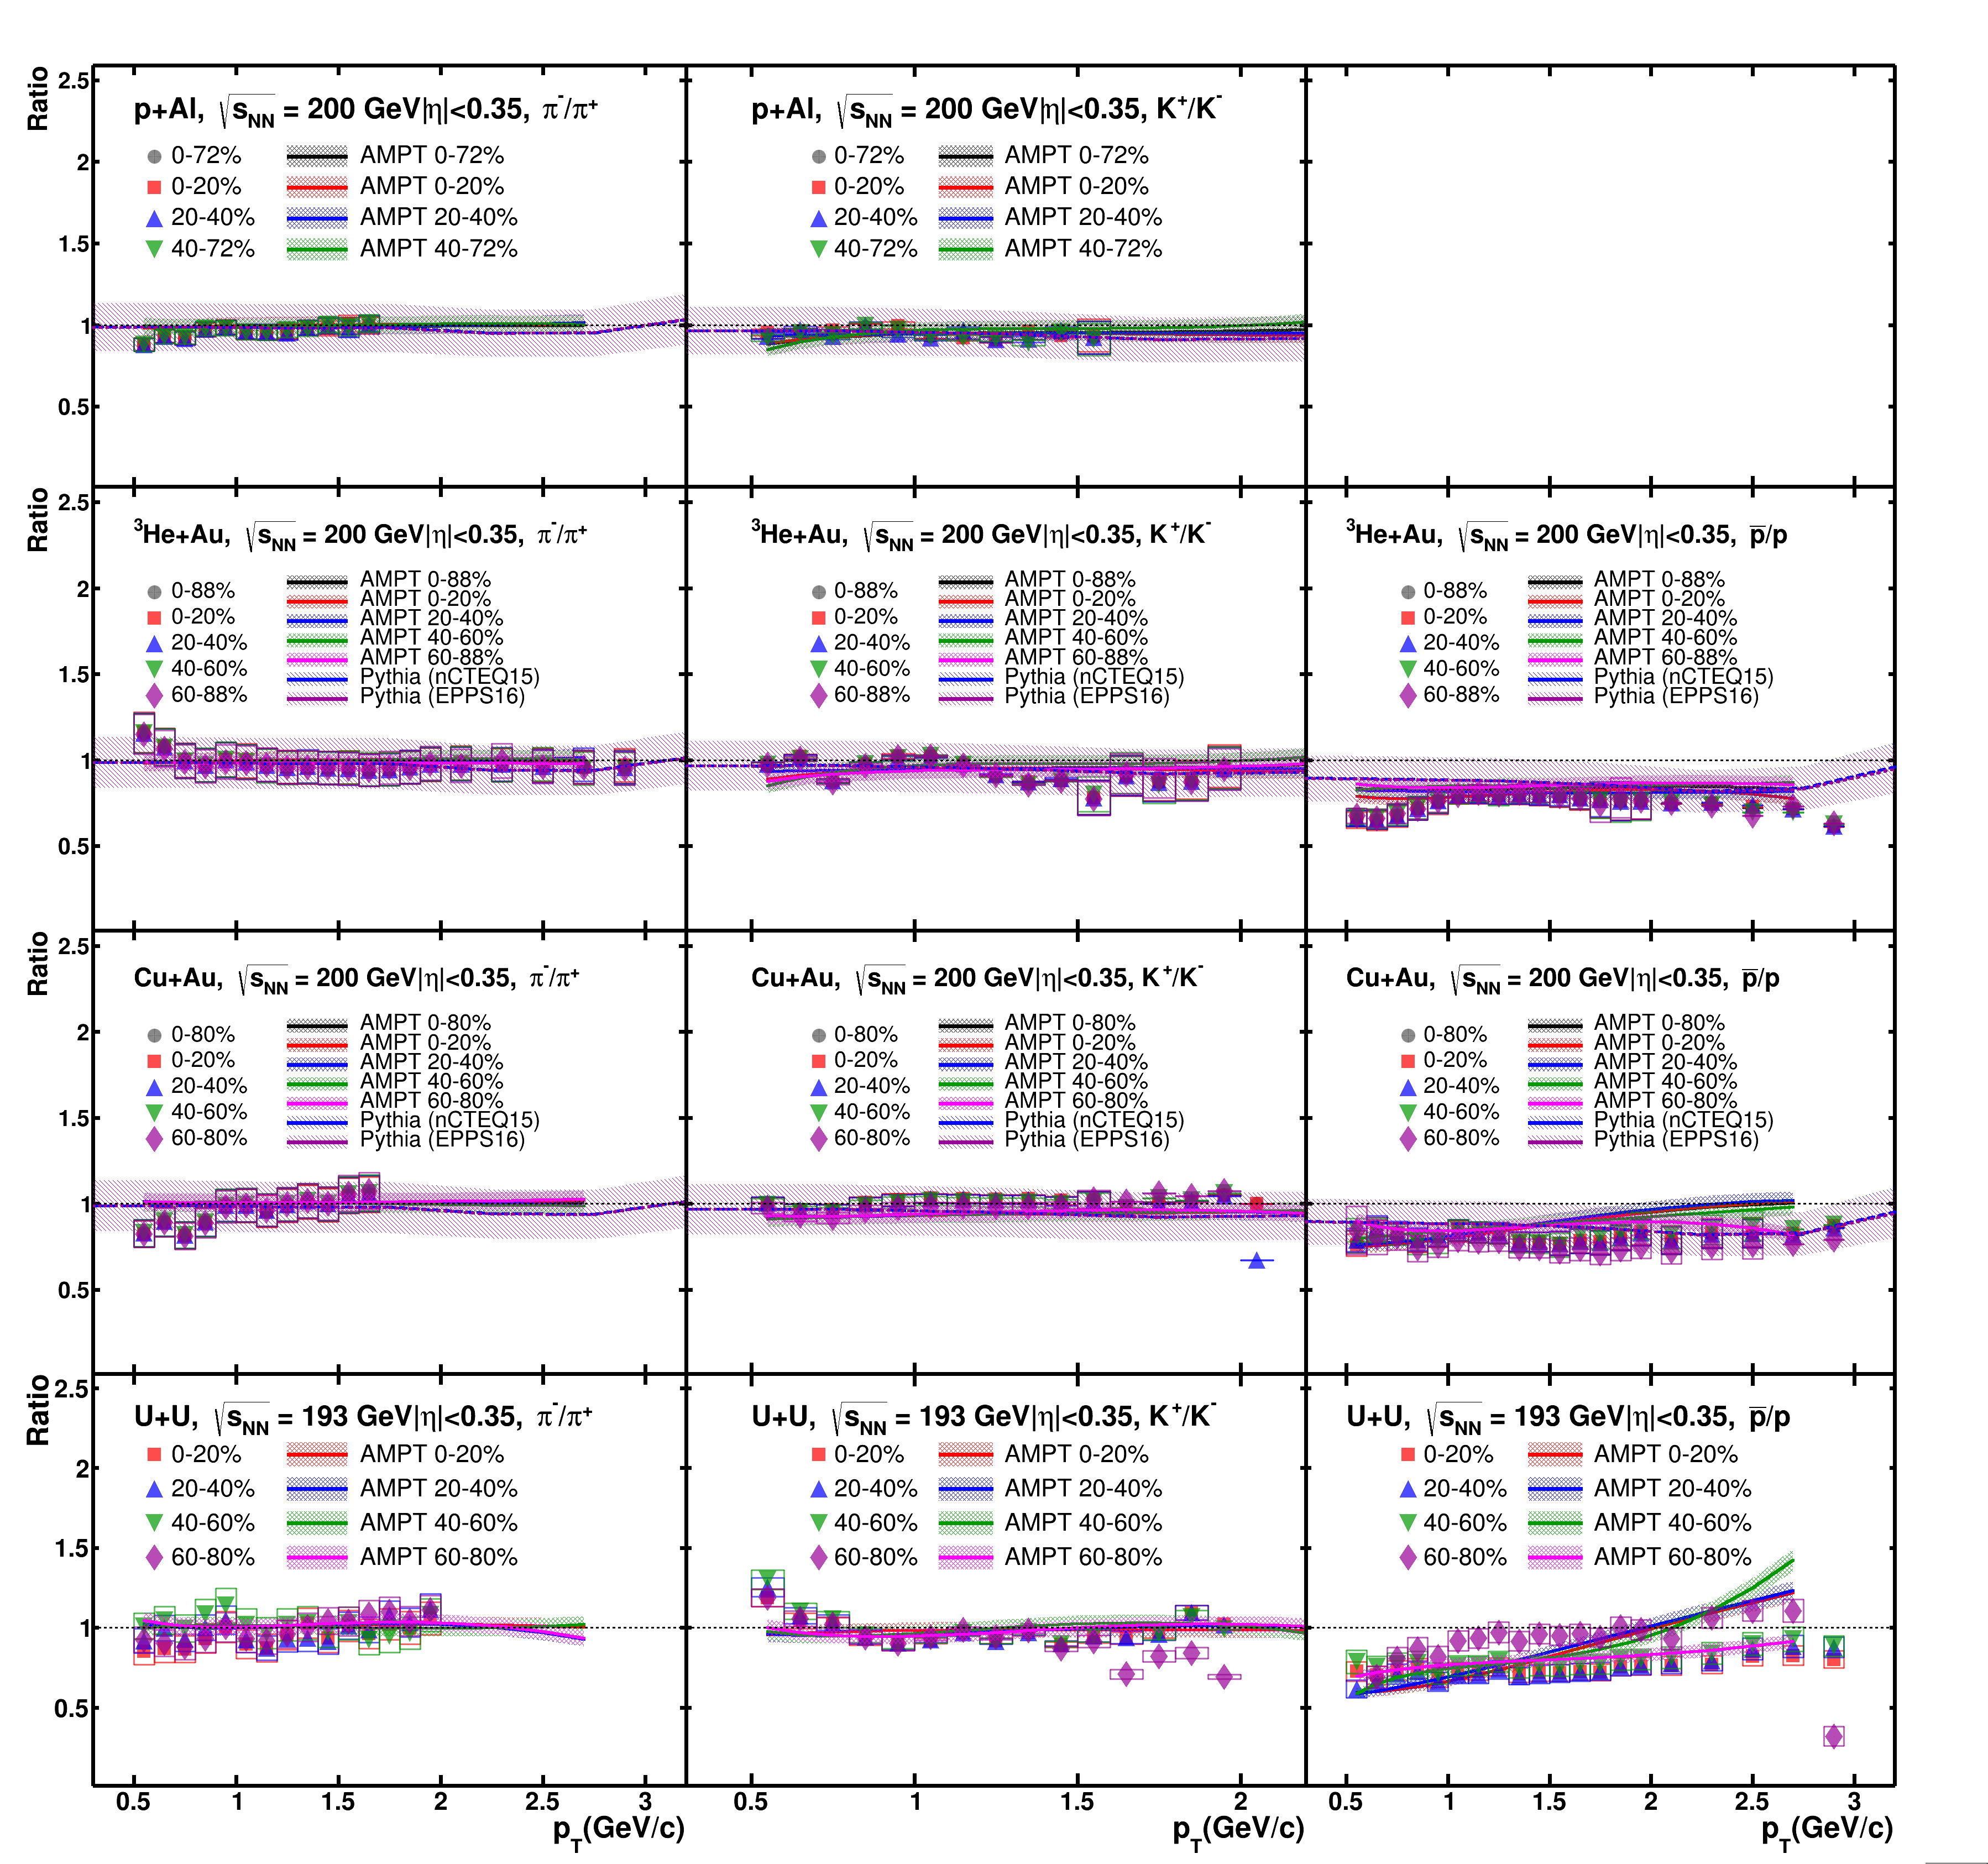
\includegraphics [width=1\linewidth]{Simulation/Ratio_same_AMPT_Pythia.png}
	\caption{Сравнение величин $\pi^{-}/\pi^{+}$, $K^{-}/K^{+}$, $\bar{p}/p$, полученных в рамках фрагментационной (Pythia8) и рекомбинационной (AMPT) моделей, с экспериментальными результатами в различных центральностях \pal, \heau, Cu+Au и U+U столкновений.} 
	\label{img:Ratio_same_sym}
\end{figure}


\begin{figure}[] 
	\centerfloat
	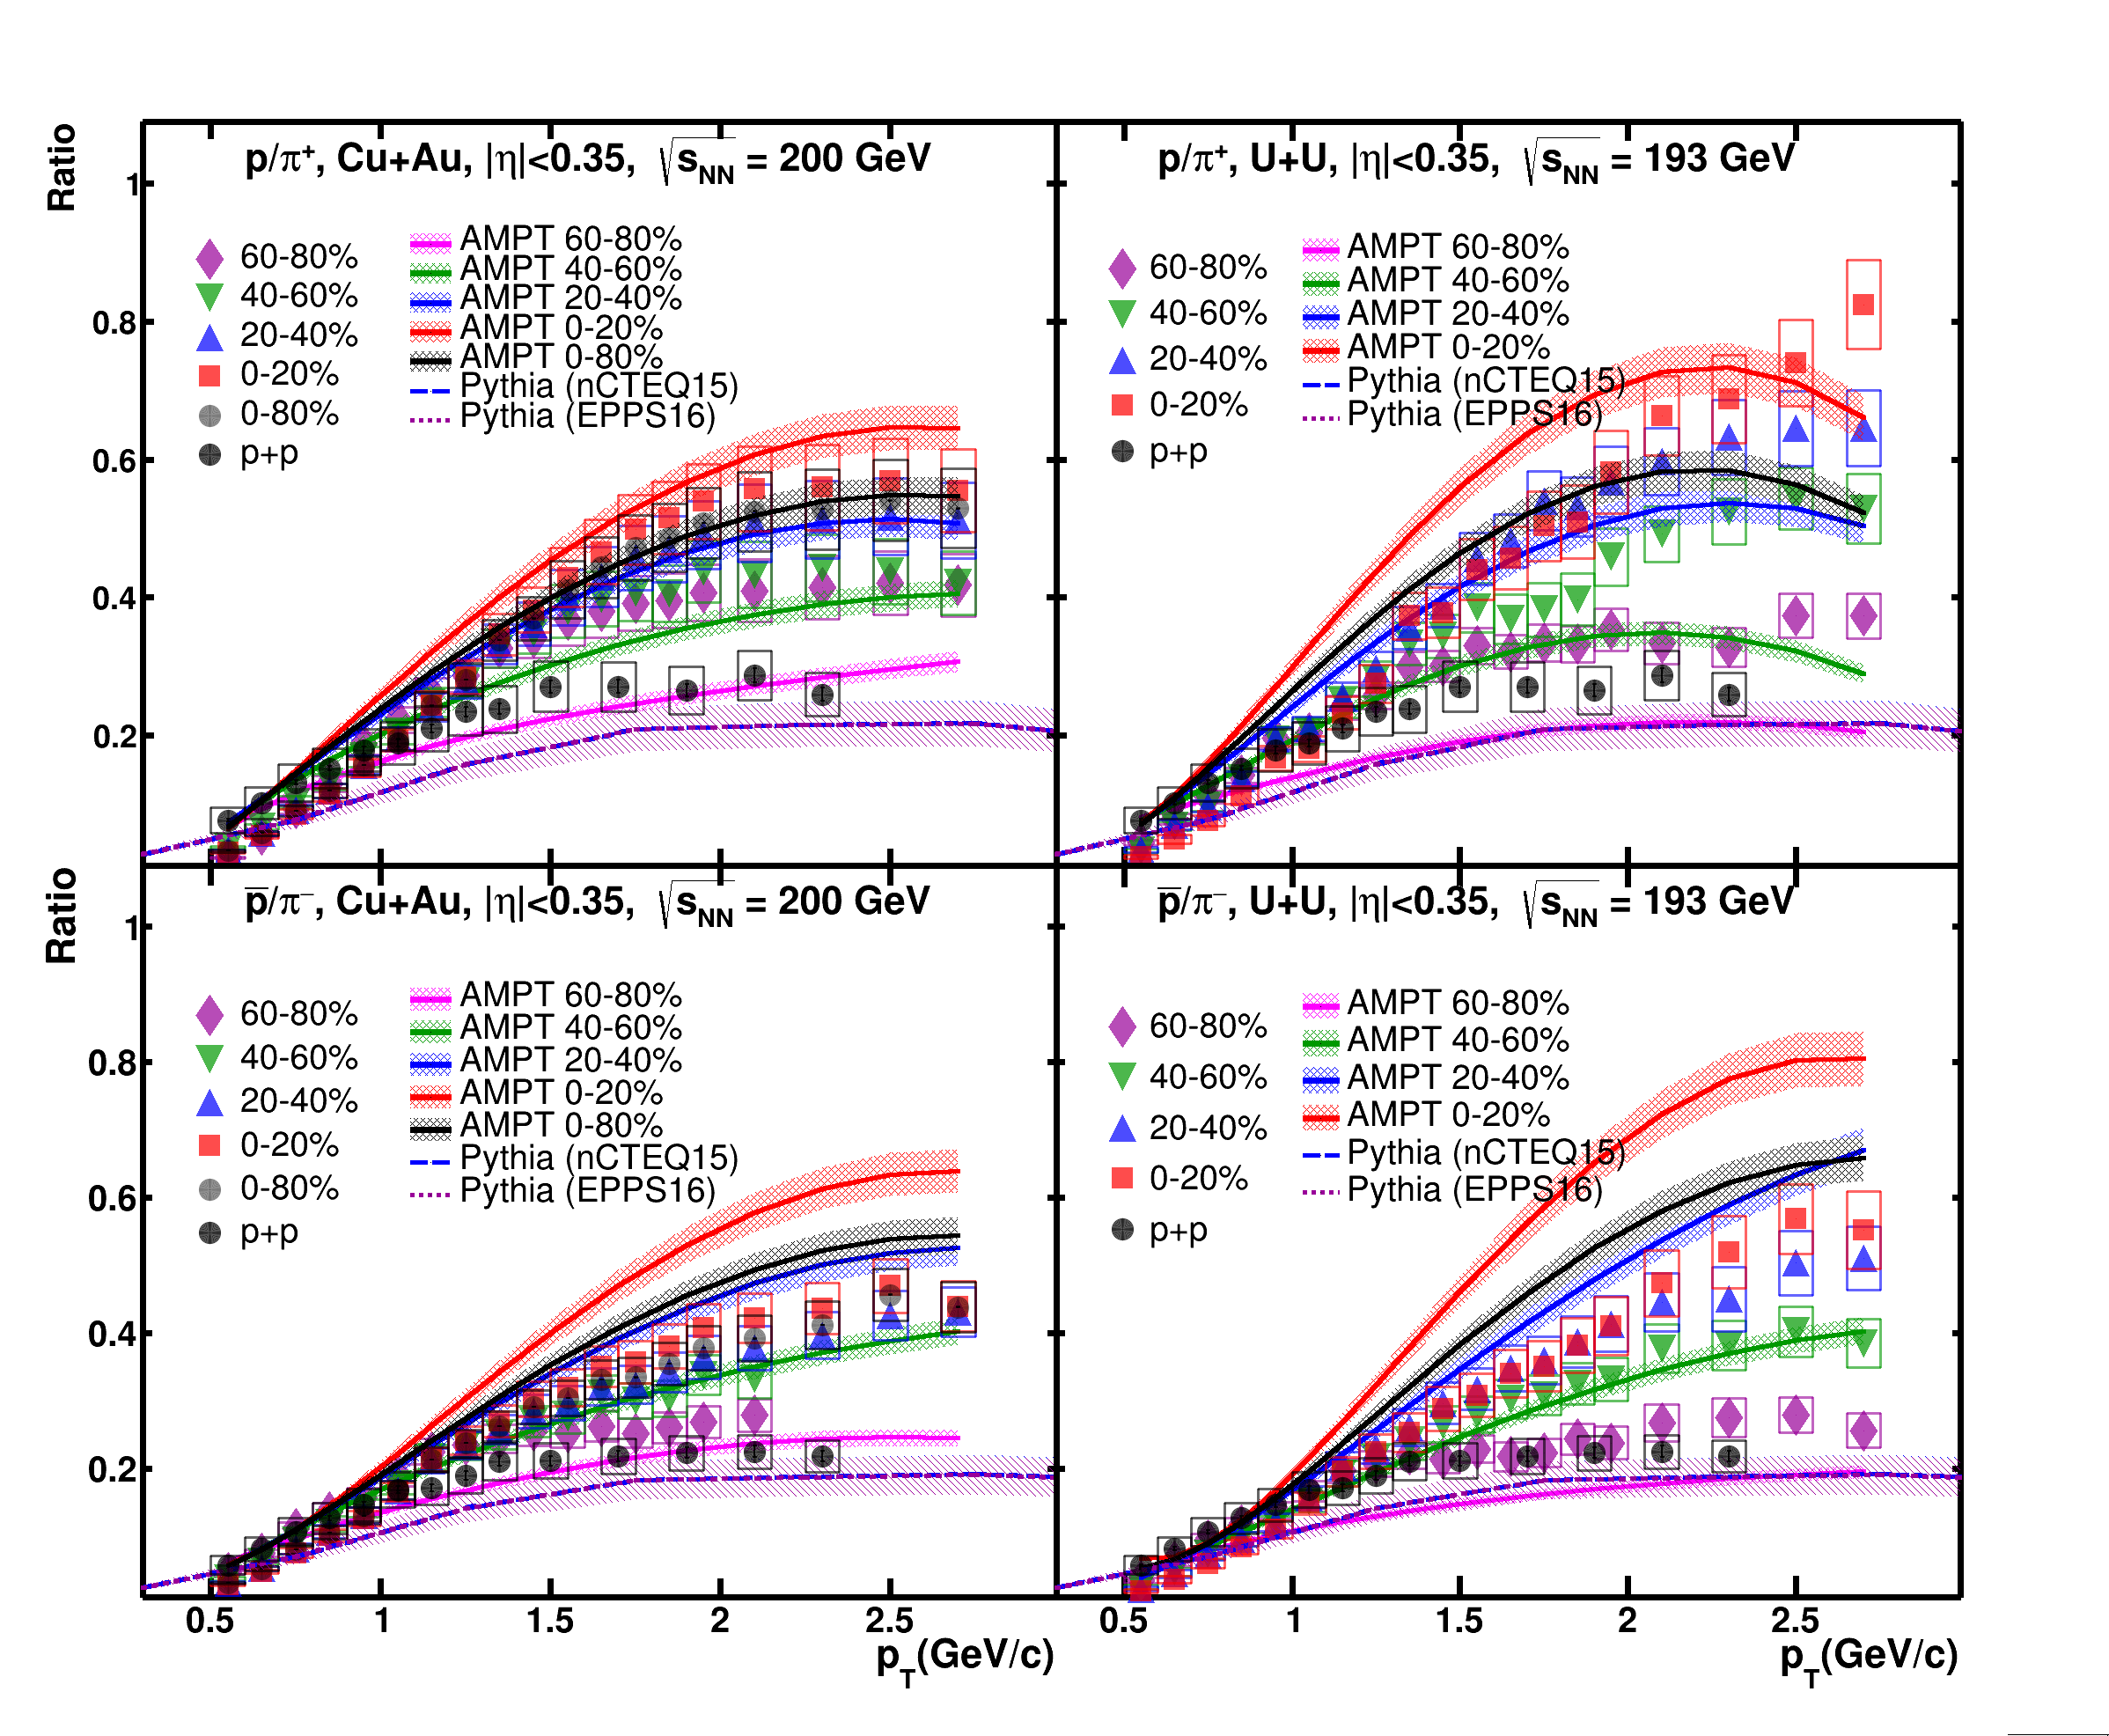
\includegraphics [width=1\linewidth]{Simulation/Ratios_AMPT_large_p2pi.png}
	\caption{Сравнение величин $p/\pi^{+}$ и $\bar{p}/\pi^{+}$, полученных в рамках фрагментационной (Pythia8) и рекомбинационной (AMPT) моделей, с экспериментальными результатами в различных центральностях Cu+Au и U+U столкновений.} 
	\label{img:Ratio_LargeP2PI_sym}
\end{figure}

\begin{figure}[] 
	\centerfloat
	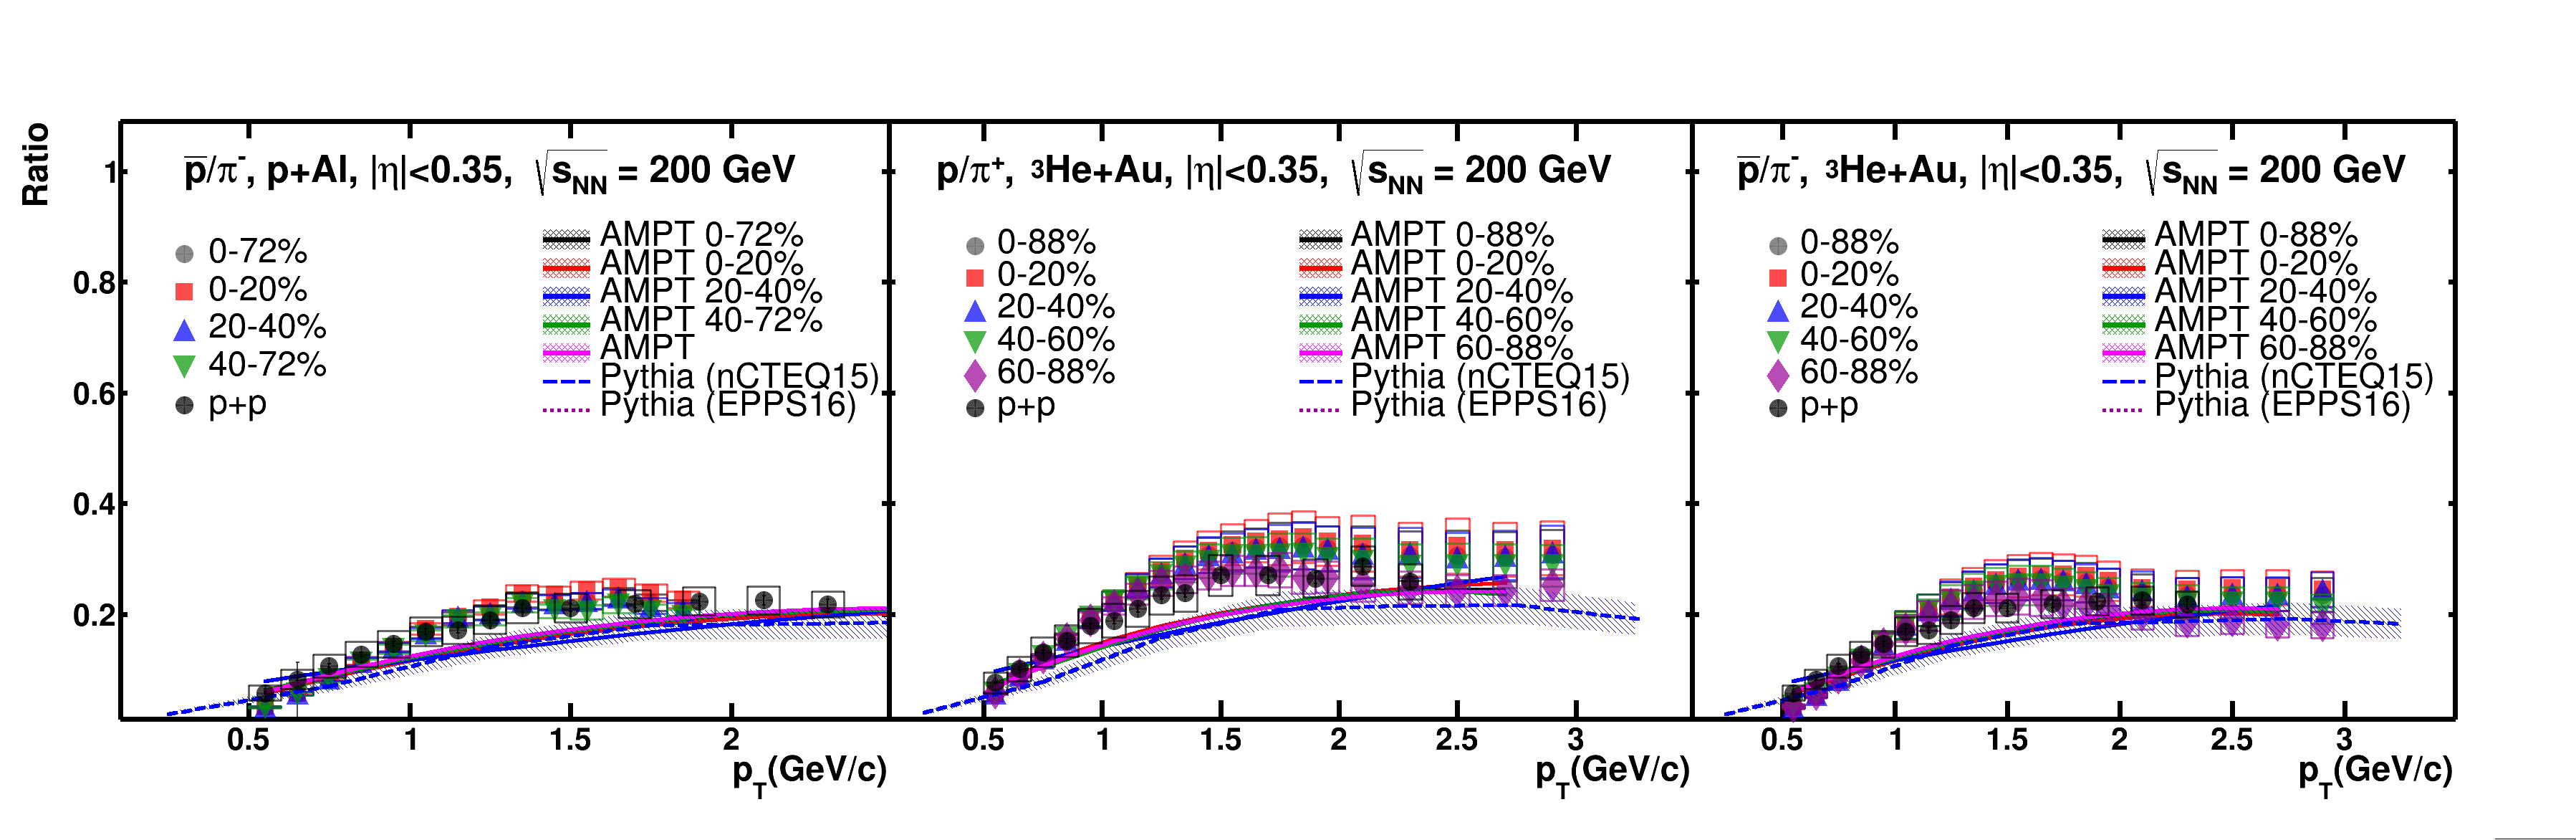
\includegraphics [width=1\linewidth]{Simulation/Ratios_AMPT_small_p2pi.png}
	\caption{Сравнение величин $p/\pi^{+}$ и $\bar{p}/\pi^{-}$, полученных в рамках фрагментационной (Pythia8) и рекомбинационной (AMPT) моделей, с экспериментальными результатами в различных центральностях \pal \ и \heau \ столкновений.} 
	\label{img:Ratio_SmallP2PI_sym}
\end{figure}

\begin{figure}[] 
	\centerfloat
	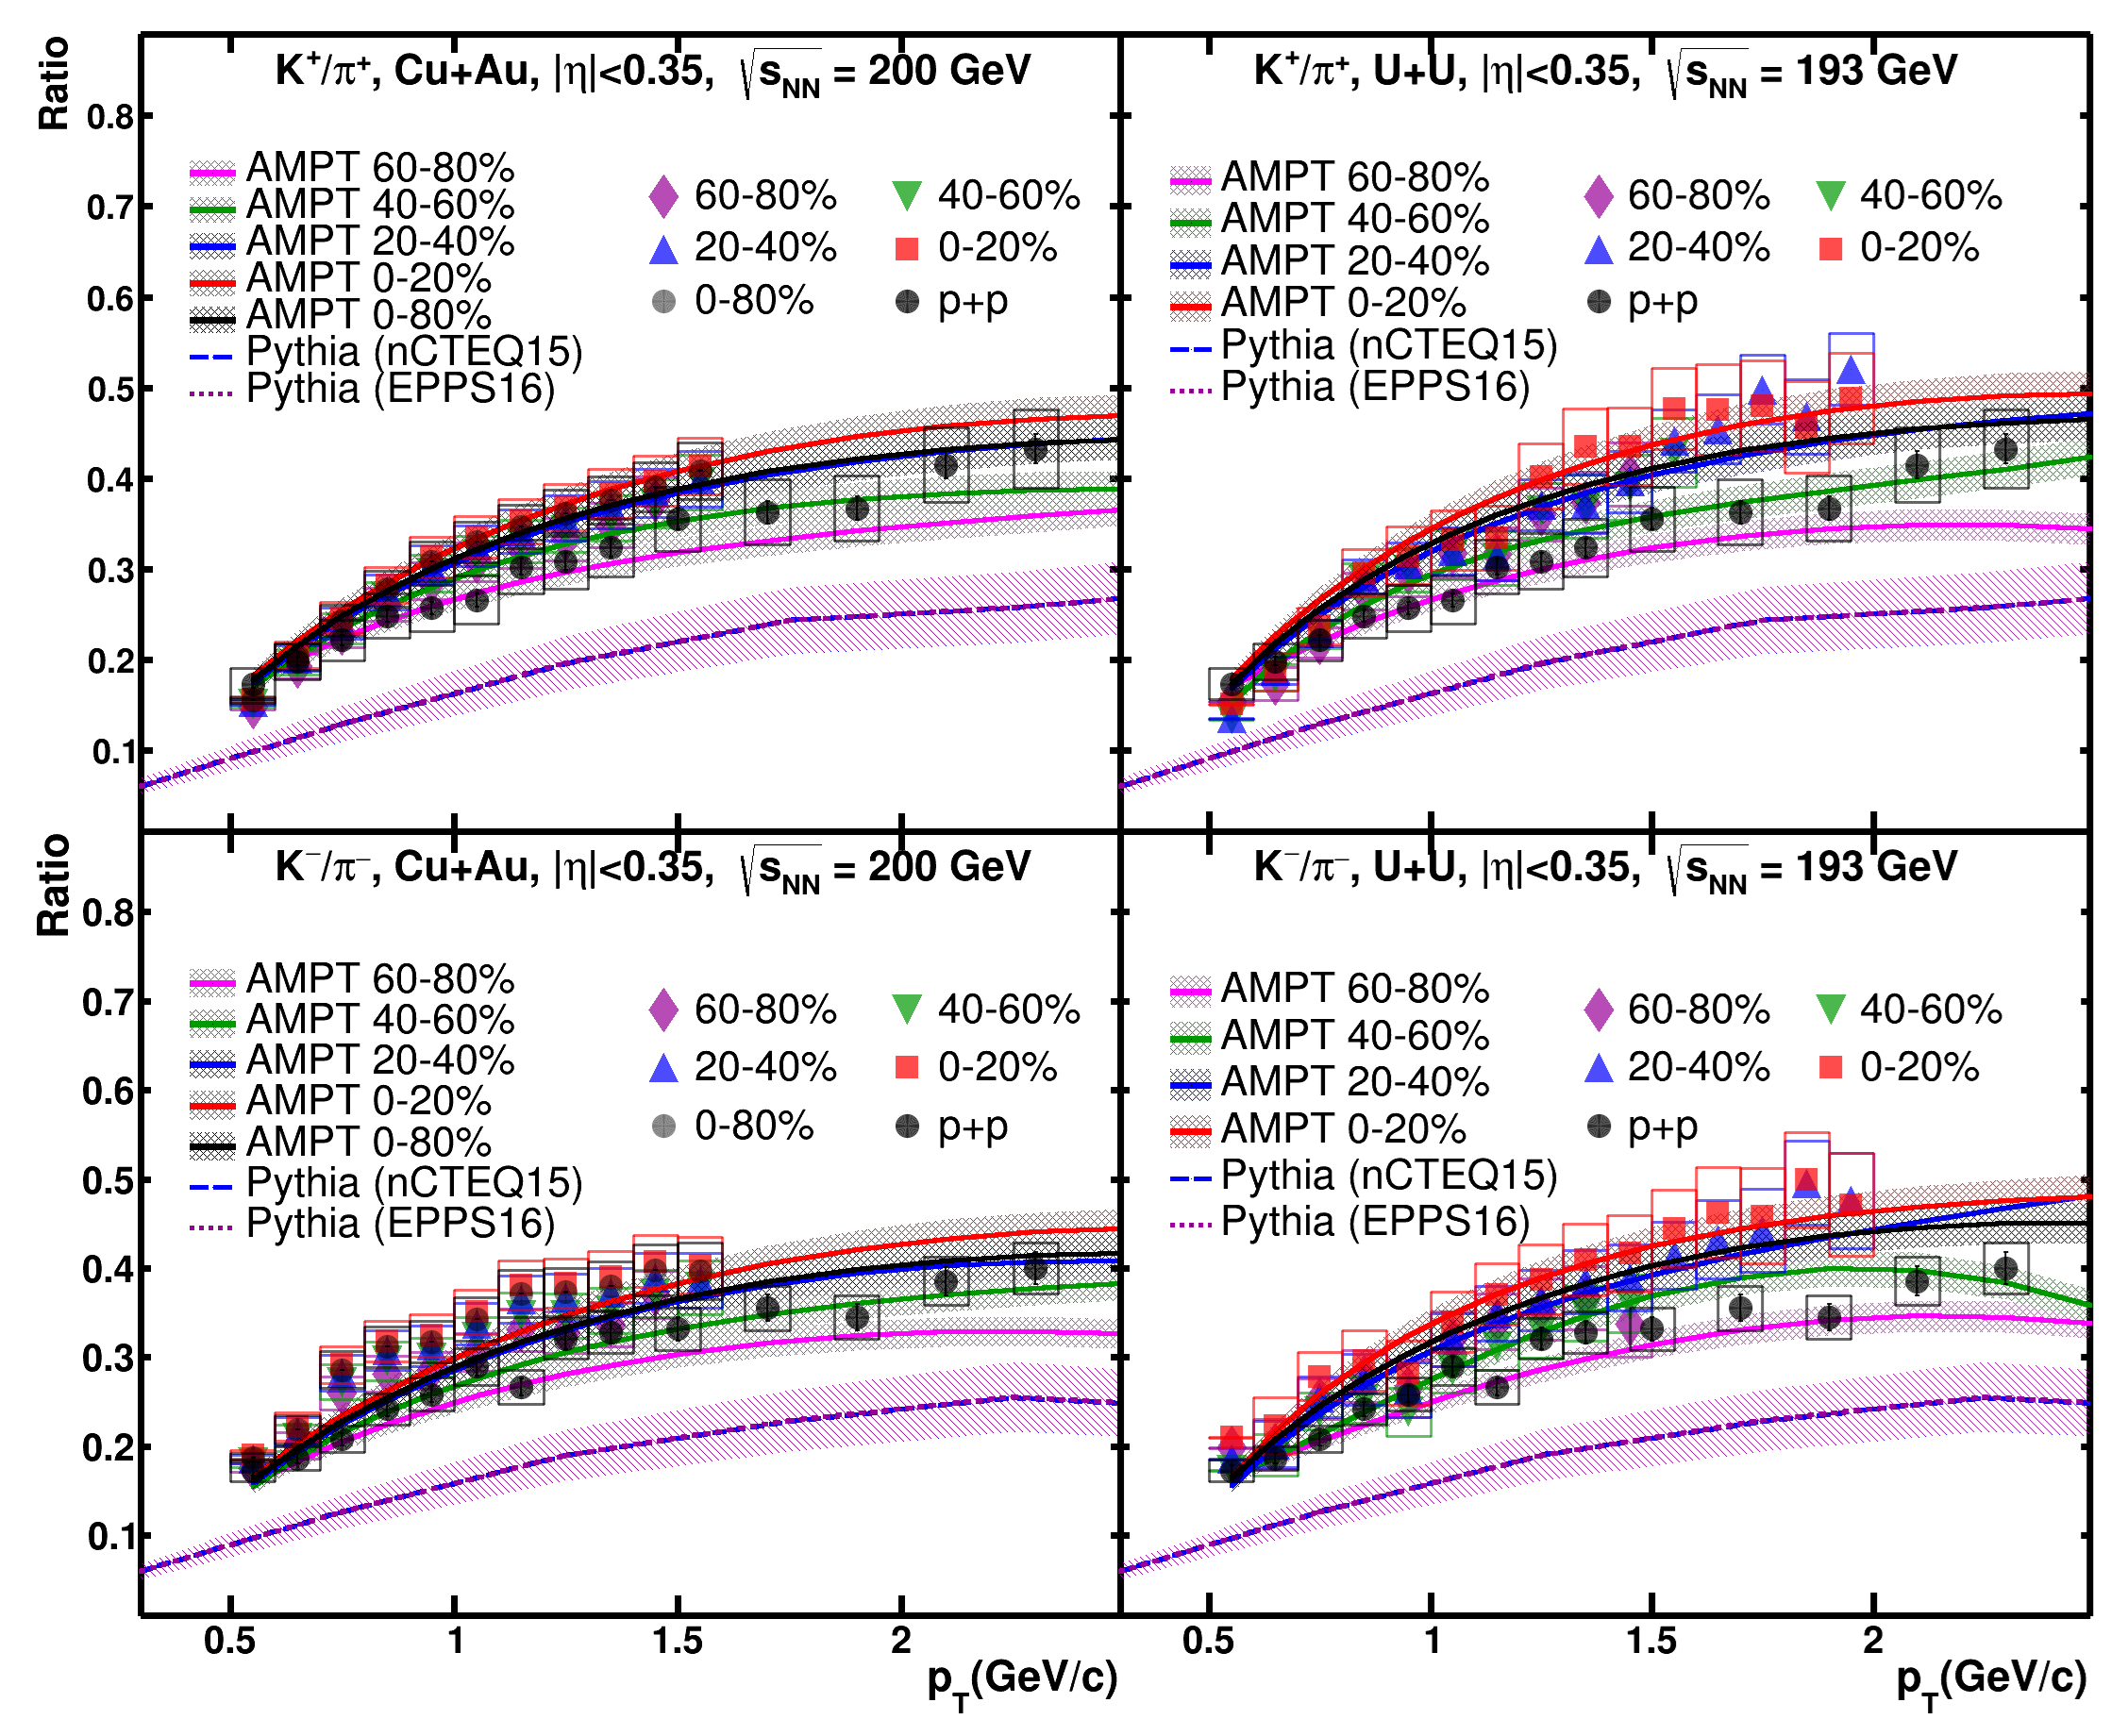
\includegraphics [width=1\linewidth]{Simulation/Ratios_AMPT_large_K2pi.png}
	\caption{Сравнение величин $K^{+}/\pi^{+}$ и $K^{-}/\pi^{-}$, полученных в рамках фрагментационной (Pythia8) и рекомбинационной (AMPT) моделей, с экспериментальными результатами в различных центральностях Cu+Au и U+U столкновений.} 
	\label{img:Ratio_LargeK2PI_sym}
\end{figure}

\begin{figure}[] 
	\centerfloat
	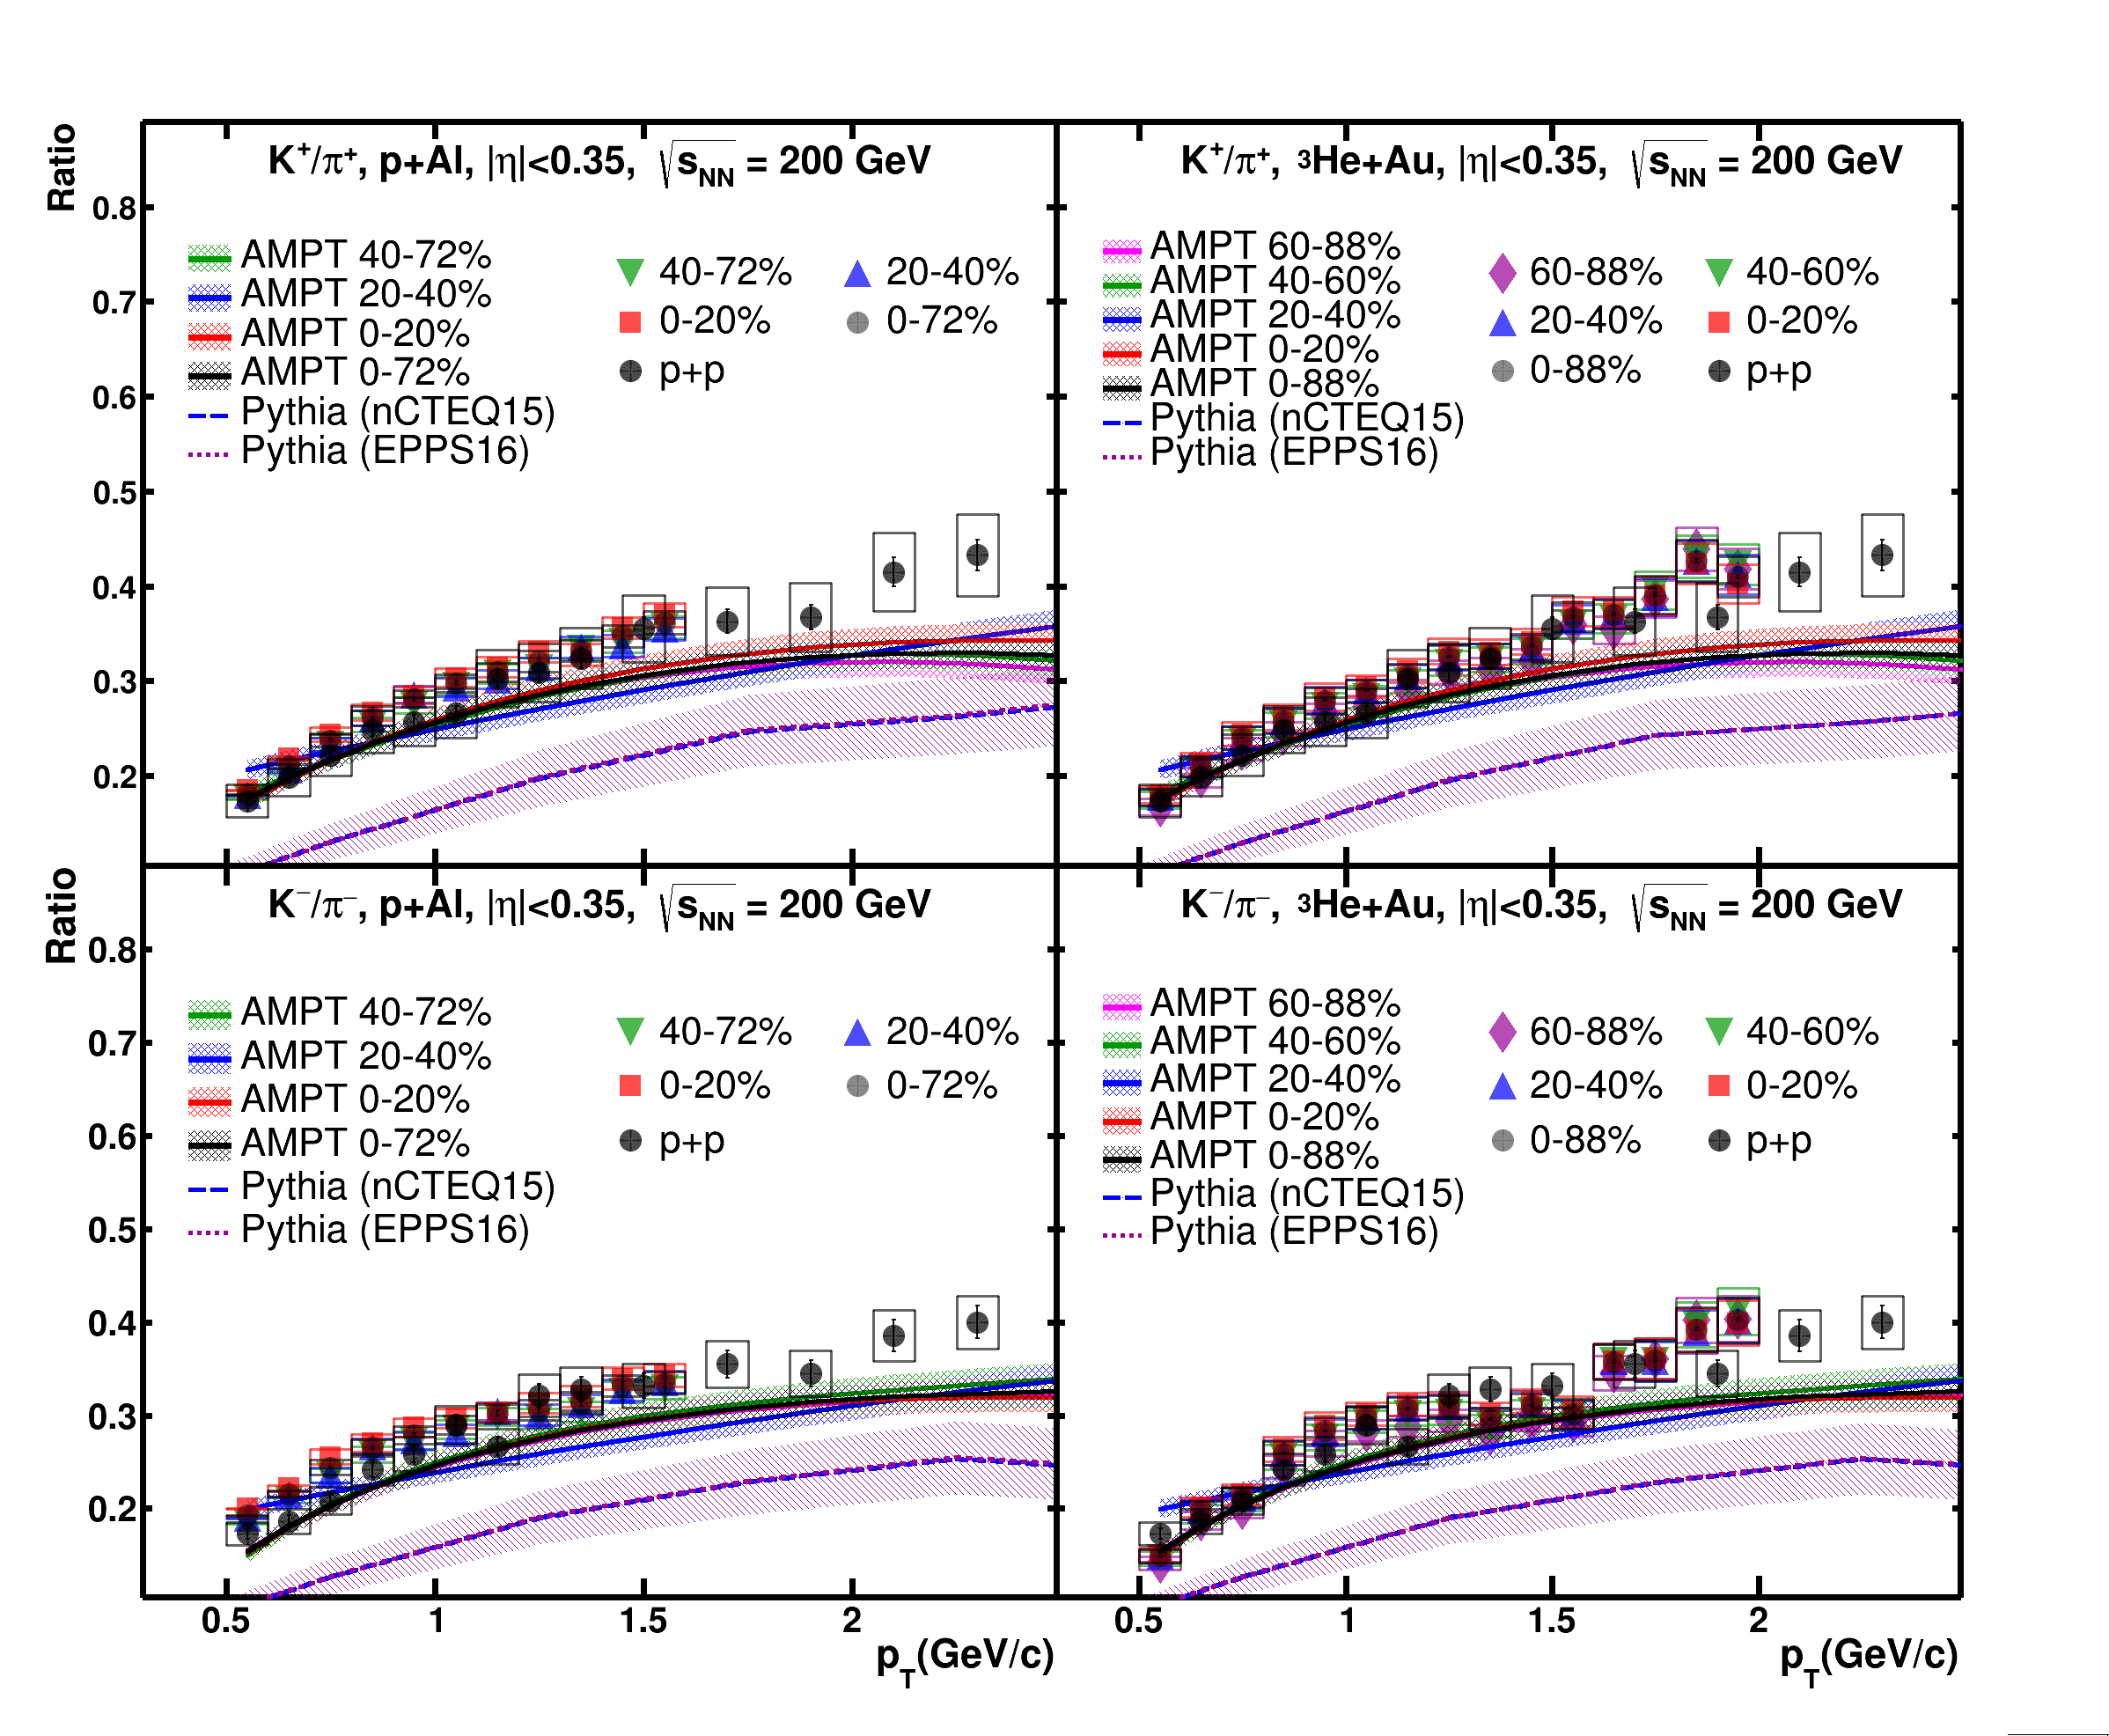
\includegraphics [width=1\linewidth]{Simulation/Ratios_AMPT_small_K2pi.png}
	\caption{Сравнение величин $K^{+}/\pi^{+}$ и $K^{-}/\pi^{-}$, полученных в рамках фрагментационной (Pythia8) и рекомбинационной (AMPT) моделей, с экспериментальными результатами в различных центральностях \pal \ и \heau \ столкновений.} 
	\label{img:Ratio_SmallK2PI_sym}
\end{figure}